% Aquí se debe definir un conjunto de pruebas que serán entregadas como 
% resultado final del proyecto y verificación del mismo. 
% Las mismas podrán ser ajustadas más adelante.

\noindent Inicialmente, partimos de la premisa de que nuestra arquitectura distribuida era naturalmente más escalable
que una arquitectura monolítica. En esta sección realizaremos diversas pruebas con distintas configuraciones de nodos del servidor y cantidad
de jugadores conectados para validar esta hipótesis. Para facilitar estas pruebas y hacerlas reproducibles, utilizaremos los Bots desarrollados
en la sección \ref{sec:Bots}. Las siguientes pruebas fueron realizadas en el entorno de Kubernetes descrito en la sección \ref{sec:lessons-kubernetes}, que es actualmente el entorno
productivo de \textit{Fiubakka}, pero es posible realizar estas pruebas sin necesidad de un ambiente de Kubernetes, mediante múltiples instancias del
servidor en una misma máquina.

A priori, lo que esperamos observar en las pruebas de carga es que el consumo de CPU sobre un único nodo de la aplicación tenga una \textbf{complejidad temporal
de $\boldsymbol{O(n^2)}$}, donde \textit{n} es la cantidad de jugadores conectados induciendo carga continua. Esto es así porque cada evento generado por un jugador debe ser procesado por todos los
demás jugadores que se encuentren en el mismo mapa. Dado que queremos forzar el peor escenario posible, todos los jugadores creados en las pruebas de carga comparten el mismo mapa.
Es importante recalcar que esta complejidad temporal es inherente a la naturaleza de la notificación de los eventos del juego a todos los jugadores, no es algo particular de nuestra arquitectura; un servidor monolítico
enfrentaría la misma complejidad temporal.

Donde nuestra aplicación se debería destacar es en la escalabilidad horizontal, y aquí entra la segunda observación que esperamos ver en los resultados de las pruebas. Dada la complejidad temporal de
$O(n^2)$ en un único nodo, esperamos que al distribuir la carga de jugadores en \textit{m} nodos para una misma \textit{n} cantidad de jugadores, el consumo de CPU por nodo será proporcional a \textbf{$\frac{n^2}{m}$}, donde \textit{m} es la cantidad de nodos
de la aplicación. En otras palabras, esperamos que el consumo de CPU por nodo disminuya en la misma proporción que la cantidad de nodos. Esta es la principal ventaja de nuestra arquitectura en comparación con las monolíticas,
además de la distribución de responsabilidades y procesamiento de los eventos a los clientes de los jugadores conectados, quitando carga de los nodos del servidor.

La relación $\frac{n^2}{m}$ de carga en cada nodo resulta intuitiva si lo llevamos al caso donde $n = m$. Si la cantidad de nodos del cluster de \textit{Fiubakka} es igual a la cantidad de jugadores conectados,
y los jugadores en consecuencia se distribuyen uniformemente entre los nodos (garantizado por el rebalanceo de entidades de Cluster Sharding) entonces cada nodo procesa los mensajes de todos los demás jugadores
únicamente para el jugador que tenga asignado. Si esta relación entre jugadores y nodos se mantiene fija para cualquier cantidad de jugadores, resultaría en una complejidad temporal de $O(n)$ por nodo, con
\textit{n} siendo la cantidad de jugadores total en el cluster.

Por supuesto, en la práctica no es el objetivo mantener el caso de $n = m$, ya que resultaría como mínimo en costos de infraestructura muy elevados y constantes inestabilidades en el sistema, pero sí es muy importante la característica de nuestra arquitectura de poder
disminuir el consumo de la aplicación en cada nodo individualmente mediante, en principio, únicamente agregar más nodos al cluster.

Como aclaración previa a las pruebas, el cluster de Kubernetes utilizado cuenta con un nodo con una CPU aproximadamente el doble de rápida que los otros dos nodos.
Todas las pruebas que involucren menos de la totalidad de los nodos únicamente utilizarán los nodos más lentos para mantener uniformidad en los resultados.
Igualmente, a los efectos del resultado esperado, es esperable que dada una utilización de CPU \textit{x} en un nodo del servidor, se reduzca aproximadamente a
$\frac{x}{m}$ donde \textit{m} es la cantidad de nodos del Akka cluster. Esta proporción es independiente de los recursos de cada nodo de Kubernetes. Por otro lado,
otro de los nodos cuenta con 4GiB de memoria RAM a diferencia de los otros dos nodos, que cuentan con 8GiB. A continuación se detalla un cuadro con los recursos disponbiles
de cada nodo.

\begin{center}
\begin{tabular}{|c|c|c|c|}
    \hline
    \textbf{Nodo} & \textbf{Núcleos del procesador} & \textbf{Velocidad del procesador} & \textbf{Memoria RAM} \\
    \hline
    raspberrypi1 & 4 & 1.8GHz & 8GiB \\
    \hline
    raspberrypi2 & 4 & 1.8GHz & 4GiB \\
    \hline
    raspberrypi3 & 4 & 2.4GHz & 8GiB \\
    \hline
\end{tabular}
\end{center}

Lógicamente, para cada prueba realizada se adjunta el nodo de Kubernetes en el que se ejecutó el \textit{pod}, para poner en referencia los recursos utilizados.

\subsection{Recursos utilizados por 1 nodo de \textit{Fiubakka}}

\noindent Comenzamos con la prueba más simple, un único nodo del cluster de \textit{Fiubakka} en \textit{idle}, esto es, sin ningún jugador conectado.
Para obtener las métricas de recursos utilizados por la aplicación debemos observar los recursos reportados por el \textbf{pod} en Kubernetes.
Es importante tener en cuenta que Kubernetes reporta el consumo de CPU en \textit{millicores}. Por ejemplo, 1000m representa 1000 \textit{millicores}, equivalente
a 1 core de la CPU del nodo de Kubernetes en el que se encuentre el pod. Kubernetes es agnóstico a la velocidad del procesador en sí, en la práctica lo que tiende a suceder
es que nodos más rápidos que otros reportan un consumo de CPU menor para la misma tarea.

El resultado obtenido es el siguiente:

\begin{table}[h]
\centering
\begin{tabular}{|c|c|c|}
    \hline
    \textbf{Nodo de ejecución} & \textbf{Consumo de CPU} & \textbf{Consumo de memoria} \\
    \hline
    raspberrypi1 & 269m & 344Mi \\
    \hline
\end{tabular}
\caption{Consumo de recursos en \textit{idle} del nodo raspberrypi1.}
\end{table}

Para demostrar el punto anterior sobre el consumo de CPU en nodos más rápidos, este es el resultado para el nodo \textbf{raspberrypi3}:

\begin{table}[h]
\centering
\begin{tabular}{|c|c|c|}
    \hline
    \textbf{Nodo de ejecución} & \textbf{Consumo de CPU} & \textbf{Consumo de memoria} \\
    \hline
    raspberrypi3 & 118m & 374Mi \\
    \hline
\end{tabular}
\caption{Consumo de recursos en \textit{idle} del nodo raspberrypi3.}
\end{table}

Vemos que es aproximadamente la mitad del consumo de CPU respecto al nodo \textbf{raspberrypi1}. Esto es coherente con lo mostrado en el cuadro de recursos de cada
nodo.

\subsection{Pruebas de carga en 1 nodo}

\noindent Procederemos a realizar pruebas de carga con distintas cantidades de jugadores, comenzando por un único nodo de la aplicación. Esto
nos dará un punto de referencia para comparar con pruebas posteriores, donde incrementaremos la cantidad de nodos y haremos una comparativa con los resultados
obtenidos en esta sección.

Como mencionamos anteriormente, todas las pruebas de carga se realizan simulando jugadores mediante el uso de Bots. Cada Bot ejercerá carga máxima posible por un único jugador, que corresponde
al caso de movimiento constante. Cuando el jugador se mueve resulta en el envío de un mensaje cada aproximadamente 16 milisegundos, siendo esta la máxima frecuencia de mensajes que el servidor
procesa por jugador.

Los resultados obtenidos fueron los siguientes:

\begin{table}[h]
\centering
\begin{tabular}{|c|c|c|c|}
    \hline
    \textbf{Nodo de ejecución} & \textbf{Cantidad de jugadores} & \textbf{Consumo de CPU} & \textbf{Consumo de memoria} \\
    \hline
    raspberrypi1 & 1 & 352m & 553Mi \\
    \hline
    raspberrypi1 & 2 & 488m & 443Mi \\
    \hline
    raspberrypi1 & 4 & 797m & 712Mi \\
    \hline
    raspberrypi1 & 8 & 1359m & 790Mi \\
    \hline
    raspberrypi1 & 16 & 2780m & 1173Mi \\
    \hline
    raspberrypi1 & 24 & 3485m & 1645Mi \\
    \hline
\end{tabular}
\caption{Consumo de recursos en 1 nodo con distintas cantidades de jugadores.}
\end{table}

Con la última prueba de carga con 24 jugadores llegamos al límite de CPU que el nodo \textbf{raspberrypi1} tolera, pasado este número estamos ejerciendo más carga que la que el procesador
puede soportar \textit{gracefully} y comienzan los errores de mensajes no entregados, por lo que nos detendremos aquí. 

En principio, pareciera que el consumo de CPU escala en el orden lineal con la cantidad de jugadores. Esto contradice nuestro planteo original
de que cada jugador introducido en el sistema induce, en el peor escenario, una incremento cuadrático en el consumo total, dado que cada evento generado se debe procesar \textit{n} veces, donde \textit{n} denota la cantidad de jugadores en el servidor.
Teniendo \textit{n} jugadores resultaría en procesar \textit{n} veces los eventos de los \textit{n} jugadores, dando lugar a la complejidad cuadrática.
Sobre este punto, nuestra hipótesis es que el comportamiento esperado únicamente se visibiliza en sistemas con muchos más recursos de CPU disponibles, donde es posible realizar pruebas de carga
con cantidades de jugadores mucho más elevadas.

Para validar esta hipótesis utilizamos una herramienta que presentaremos más detalladamente en una próxima sección, pero que por ahora alcanza con entender que los siguientes gráficos corresponden a la cantidad de eventos generados entre todos los jugadores
y la cantidad de eventos procesados en total por todos los jugadores, respectivamente. A medida que el tiempo avanza se agregan jugadores al sistema, a ritmo constante, donde cada uno genera la misma cantidad de eventos que los demás.

\begin{figure}[htbp]
    \centering
    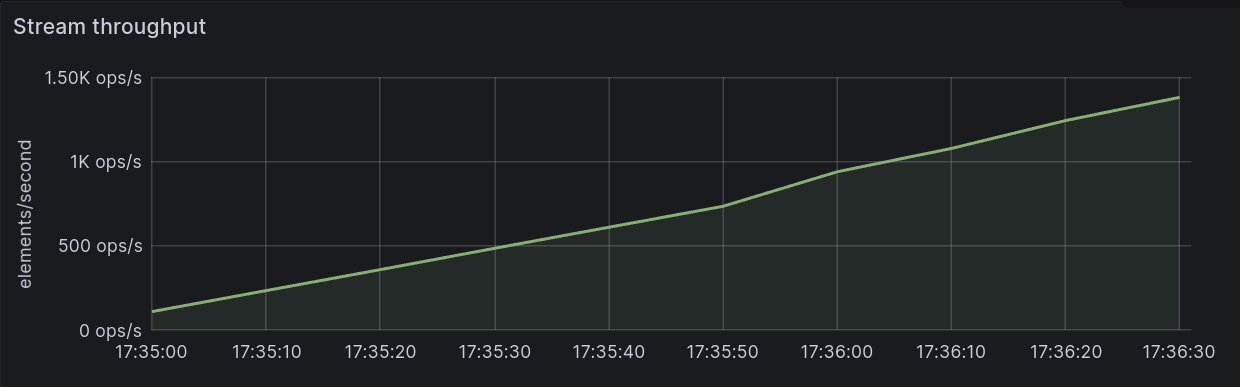
\includegraphics[width=1\textwidth]{../assets/stream-producer-metrics.png}
    \caption{Procesamiento de eventos generados en función de la cantidad de jugadores.}
\end{figure}

\begin{figure}[htbp]
    \centering
    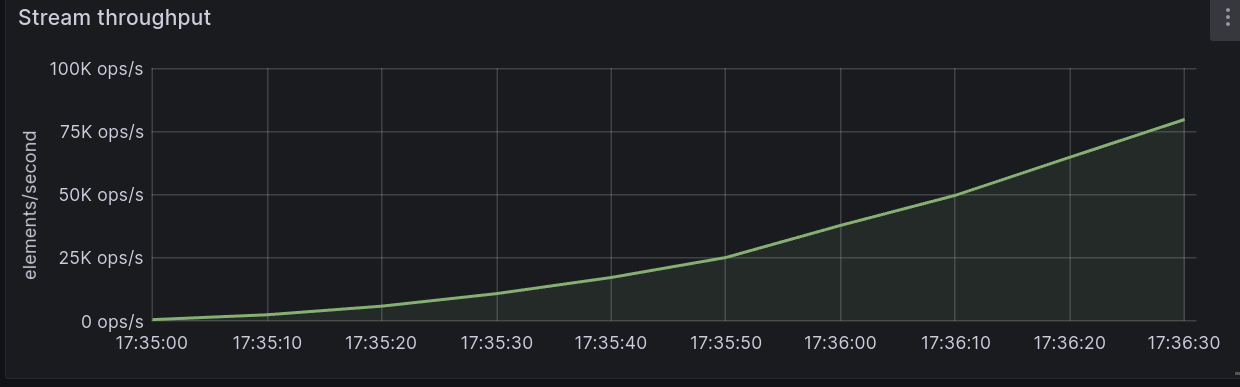
\includegraphics[width=1\textwidth]{../assets/stream-consumer-metrics.png}
    \caption{Procesamiento de eventos consumidos en función de la cantidad de jugadores.}
\end{figure}

Vemos que para el caso de los eventos generados tenemos claramente una tendencia lineal, esperable dado que cada jugador introducido genera la misma cantidad de eventos en el sistema independientemente de los demás jugadores.
Para los eventos consumidos en cambio vemos que la pendiente no es lineal, y se puede apreciar lo que parece una asíntota más cuadrática. Si reducimos la resolución y observamos ambas mediciones en un rango de tiempo más amplio,
los resultados son más claros.

\begin{figure}[htbp]
    \centering
    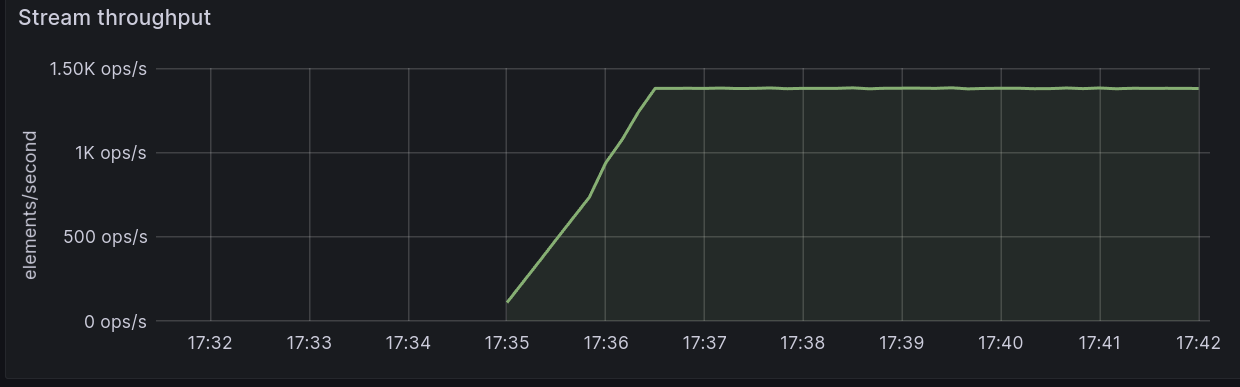
\includegraphics[width=1\textwidth]{../assets/stream-producer-amplified-metrics.png}
    \caption{Procesamiento de eventos generados en función de la cantidad de jugadores.}
\end{figure}

\begin{figure}[htbp]
    \centering
    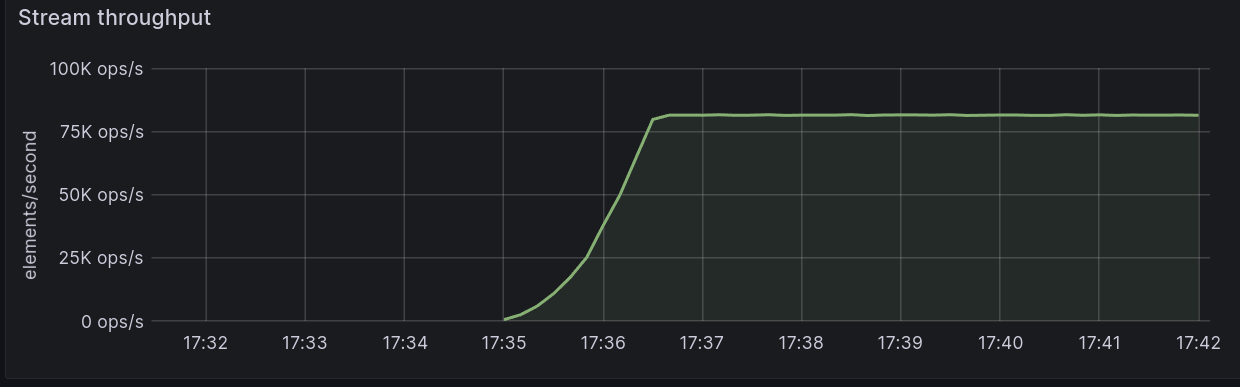
\includegraphics[width=1\textwidth]{../assets/stream-consumer-amplified-metrics.png}
    \caption{Procesamiento de eventos consumidos en función de la cantidad de jugadores.}
\end{figure}

El hecho de que ambas métricas se mantengan constantes a partir de cierto punto se debe a que ese es el momento en el que se deja de agregar jugadores al sistema, manteniendo la carga
constante de allí en adelante. Validamos entonces nuestra hipótesis original respecto a la complejidad temporal de la aplicación en un único nodo.

Con esto concluimos el análisis de escalabilidad vertical de nuestra aplicación. En la siguiente sección evaluaremos las métricas obtenidas
con más de un nodo del cluster de \textit{Fiubakka} para validar la hipótesis de escalabilidad horizontal.

\subsection{Pruebas de carga en múltiples nodos (RaspberryPi)}

\noindent Habiendo medido el consumo de recursos de la aplicación para múltiples configuraciones de jugadores en un único nodo, realizaremos ahora las mismas configuraciones de jugadores totales
pero distribuidos en más de un nodo uniformemente. La idea es que, si la aplicación es escalable horizontalmente, el consumo de recursos por nodo debería ser menor que el obtenido en la sección anterior.
En la teoría, lo esperado es que el consumo de recursos en cada nodo sea proporcional a $\frac{N}{m}$, donde \textit{N} es la cantidad de jugadores en el servidor (fijado a constante) y \textit{m} es la cantidad de nodos de \textit{Fiubakka}.
Además, vamos a medir nuevamente el consumo para el caso \textit{idle} (N = 0). Dado que ahora tendremos más de un nodo en el cluster, entran en juego mecanismos de \textit{heartbeat} y comunicación
entre nodos que pueden incrementar el consumo de recursos.

Los resultados obtenidos para $m=2$, con cada nodo de \textit{Fiubakka} en un nodo distinto de Kubernetes, fueron los siguientes:

\begin{table}[h]
\centering
\begin{tabularx}{\textwidth} { 
    | >{\centering\arraybackslash}X 
    | >{\centering\arraybackslash}X 
    | >{\centering\arraybackslash}X 
    | >{\centering\arraybackslash}X | }
        \hline
        \textbf{Cantidad de jugadores (N)} & \textbf{Nodo de ejecución} & \textbf{Consumo de CPU} & \textbf{Consumo de memoria} \\
        \hline
        \multirow{2}{*}{0} & raspberrypi1 & 755m & 511Mi \\
        \cline{2-4}
        & raspberrypi2 & 744m & 549Mi \\
        \hline
        \multirow{2}{*}{2} & raspberrypi1 & 1562m & 760Mi \\
        \cline{2-4}
        & raspberrypi2 & 1487m & 642Mi \\
        \hline
        \multirow{2}{*}{4} & raspberrypi1 & 1780m & 886Mi \\
        \cline{2-4}
        & raspberrypi2 & 1850m & 692Mi \\
        \hline
        \multirow{2}{*}{8} & raspberrypi1 & 2367m & 926Mi \\
        \cline{2-4}
        & raspberrypi2 & 2247m & 732Mi \\
        \hline
        \multirow{2}{*}{16} & raspberrypi1 & 2962m & 1039Mi \\
        \cline{2-4}
        & raspberrypi2 & 3053m & 897Mi \\
        \hline
        \multirow{2}{*}{24} & raspberrypi1 & 2947m & 1105Mi \\
        \cline{2-4}
        & raspberrypi2 & 2979m & 1328Mi \\
        \hline
\end{tabularx}
\caption{Consumo de recursos en 2 nodos con distintas cantidades de jugadores.}
\end{table}

Para $m=3$ se elimina el caso de 2 jugadores, dado que no se aprovecharía la distribución entre los 3 nodos, y se modifican algunas pruebas para que
la cantidad de jugadores sea uniformemente distribuible entre los nodos. Se obtuvieron los siguientes resultados:

\begin{table}[h]
\centering
\begin{tabularx}{\textwidth} { 
    | >{\centering\arraybackslash}X 
    | >{\centering\arraybackslash}X 
    | >{\centering\arraybackslash}X 
    | >{\centering\arraybackslash}X | }
        \hline
        \textbf{Cantidad de jugadores (N)} & \textbf{Nodo de ejecución} & \textbf{Consumo de CPU} & \textbf{Consumo de memoria} \\
        \hline
        \multirow{3}{*}{0} & raspberrypi1 & 961m & 763Mi \\
        \cline{2-4}
        & raspberrypi2 & 893m & 729Mi \\
        \cline{2-4}
        & raspberrypi3 & 509m & 738Mi \\
        \hline
        \multirow{3}{*}{3} & raspberrypi1 & 1728m & 893Mi \\
        \cline{2-4}
        & raspberrypi2 & 1333m & 814Mi \\
        \cline{2-4}
        & raspberrypi3 & 1236m & 849Mi \\
        \hline
        \multirow{3}{*}{9} & raspberrypi1 & 2433m & 956Mi \\
        \cline{2-4}
        & raspberrypi2 & 1701m & 888Mi \\
        \cline{2-4}
        & raspberrypi3 & 1636m & 863Mi \\
        \hline
        \multirow{3}{*}{15} & raspberrypi1 & 2878m & 1159Mi \\
        \cline{2-4}
        & raspberrypi2 & 2828m & 982Mi \\
        \cline{2-4}
        & raspberrypi3 & 1738m & 970Mi \\
        \hline
        \multirow{3}{*}{24} & raspberrypi1 & 3058m & 1285Mi \\
        \cline{2-4}
        & raspberrypi2 & 3179m & 1265Mi \\
        \cline{2-4}
        & raspberrypi3 & 2378m & 1166Mi \\
        \hline
\end{tabularx}
\caption{Consumo de recursos en 3 nodos con distintas cantidades de jugadores.}
\end{table}

Los resultados obtenidos en principio son sorpresivos, dado que no coinciden con la hipótesis propuesta. Vemos que para cantidades bajas de jugadores
el consumo de CPU es mayor que en el caso de un único nodo, mientras que el consumo de memoria se mantiene aproximadamente igual. Para cantidades de jugadores más elevadas,
como 16 o 24, el consumo de CPU disminuye ligeramente en las configuraciones de multinodo y ya si se observa menor consumo de memoria que en el caso de un único nodo.

La explicación de este fenómeno tiene más de una arista. En primer lugar, si bien la comunicación entre actores a nivel código es transparente ya sea un único nodo o varios, no es despreciable
el hecho de que los mensajes pasan de enviarse dentro de la misma JVM a enviarse a través de la red. En el primer caso, el proceso de enviado de mensajes se reduce básicamente a una \textit{queue}
protegida mediante un \textit{mutex}, donde los mensajes se encolan y desencolan con el único \textit{overhead} siendo la adquisición del mutex.
En el segundo caso, se introduce un proceso de serialización y deserialización de los mensajes de Akka, además del \textit{overhead} que agrega el procesamiento de los paquetes
TCP y UDP a través de donde se terminan enviando los mensajes entre los nodos. La comunicación entre nodos a través de la red resulta en una carga adicional relevante, y esto es muy notorio
en el caso de pocos jugadores.

Basándonos en esta nueva hipótesis como motivo de los resultados obtenidos, y observando que para el caso de 24 jugadores particularmente \textbf{pareciera} empezar a verse una tendencia de disminución
en el uso de recursos por nodo, realizamos otra prueba en una máquina considerablemente más potente.

\subsection{Pruebas de carga en múltiples nodos (Virtualización)}
\label{sec:virtualization}

\noindent Lamentablemente no contamos con un cluster de Kubernetes con nodos más potentes para poder validar nuestra hipótesis. Si bien existen proveedores Cloud de Kubernetes como AWS, Azure o Google que
permiten configurar clusters con nodos dotados de muchos más recursos, sus costos son prohibitivos para nosotros. Sin embargo, no necesitamos formar un cluster real de Kubernetes para validar nuestra hipótesis.
Podemos formar un cluster local con nodos virtuales en una misma máquina, y realizar las pruebas de carga en dicho cluster. Siempre y cuando la máquina donde realizemos las pruebas tenga más recursos que la combinación
de las RaspberryPi, deberíamos observar una mejor performance en las pruebas de carga.

Para formar un cluster de Kubernetes virtualizado utilizamos \textbf{k3d}, dado que es una versión \textit{dockerizada} de \textit{k3s}. \textit{k3s} es la distribución de Kubernetes que utilizamos en las RaspberryPi, por
lo que garantizamos así que las pruebas sean lo más fiel posible a nuestro entorno productivo. Con \textit{k3d} podemos crear clusters de Kubernetes multinodo en una misma máquina, donde cada nodo se ejecuta como un contenedor.

A continuación se listan las características más relevantes de la máquina donde se realizaron las pruebas:

\begin{table}[h]
\centering
\begin{tabularx}{\textwidth} { 
    | >{\centering\arraybackslash}X 
    | >{\centering\arraybackslash}X 
    | >{\centering\arraybackslash}X 
    | >{\centering\arraybackslash}X | }
    \hline
    \textbf{Modelo del procesador} & \textbf{Hilos del procesador} & \textbf{Velocidad del procesador} & \textbf{Memoria RAM} \\
    \hline
    Intel i7-12700K & 20 & 4.7GHz & 32GiB \\
    \hline
\end{tabularx}
\caption{Características de la máquina utilizada para las pruebas de carga virtualizadas.}
\end{table}

Para las pruebas de carga en este entorno utilizamos un total de 84 jugadores. Esta cantidad de jugadores es divisible entre 2 y 3 nodos
uniformemente y resulta una carga adecuada para ejercer presión sobre los nodos pero no sobrecargarlos.

En este caso, todos los nodos son equivalentes en recursos, ya que comparten el mismo \textit{host}. Los resultados obtenidos fueron los siguientes:

\begin{table}[h]
\centering
\begin{tabularx}{\textwidth} { 
    | >{\centering\arraybackslash}X 
    | >{\centering\arraybackslash}X 
    | >{\centering\arraybackslash}X 
    | >{\centering\arraybackslash}X | }
        \hline
        \textbf{Cantidad de jugadores (N)} & \textbf{Nodo de ejecución} & \textbf{Consumo de CPU} & \textbf{Consumo de memoria} \\
        \hline
        84 & k3d nodo 1 & 11678m & 2396Mi \\
        \hline
        \multirow{2}{*}{84} & k3d nodo 1 & 7169m & 2091Mi \\
        \cline{2-4}
        & k3d nodo 2 & 6944m & 1958Mi \\
        \hline
        \multirow{3}{*}{84} & k3d nodo 1 & 5948m & 1905Mi \\
        \cline{2-4}
        & k3d nodo 2 & 5944m & 1672Mi \\
        \cline{2-4}
        & k3d nodo 3 & 5563m & 1588Mi \\
        \hline
\end{tabularx}
\caption{Consumo de recursos en 2 y 3 nodos virtualizados con 84 jugadores.}
\end{table}

Los resultados obtenidos ahora son prometedores, y se ajustan a la hipótesis planteada. Vemos que al distribuir la carga de los jugadores
sobre 2 nodos reducimos el consumo de CPU en aproximadamente un 40\% por nodo, y al distribuir la carga sobre 3 nodos reducimos el consumo de CPU en aproximadamente un 50\% por nodo.
Es posible que la reducción de consumo de CPU en 3 nodos sea en realidad mayor a la observada, dado que para esa configuración el procesador del \textit{host} se encontraba al 100\% de uso,
por lo que podíamos estar ante \textit{throttling}. Por otro lado, es lógico igualmente que la reducción práctica no coincida exactamente con la planteada en la teoría, ya estamos ignorando el \textit{overhead} introducido por la comunicación entre los nodos del cluster.

Por otro lado, vemos que la memoria consumida se reduce apreciablemente para la mayoría de los nodos. El nodo con consumo de memoria más elevado es, seguramente, el que tiene
asignado los Shard Coordinators de las entidades. Sería esperable que si aumentásemos la cantidad de jugadores la diferencia relativa en uso de memoria se reduzca incluso más, pero en nuestras pruebas
incrementar la cantidad de jugadores a números considerablemente más elevados ya comienza a resultar en errores en los jugadores, por lo que no pudimos verificarlo.

Finalmente, lo que sí debería verse claramente es como al aumentar la cantidad de nodos la carga de consumidores inducida en cada nodo debería ser proporcional a $\frac{n^2}{m}$.
Como referencia primero se muestra el gráfico de carga de procesamiento de eventos para el caso de un único nodo con los 84 jugadores.

\begin{figure}[htbp]
    \centering
    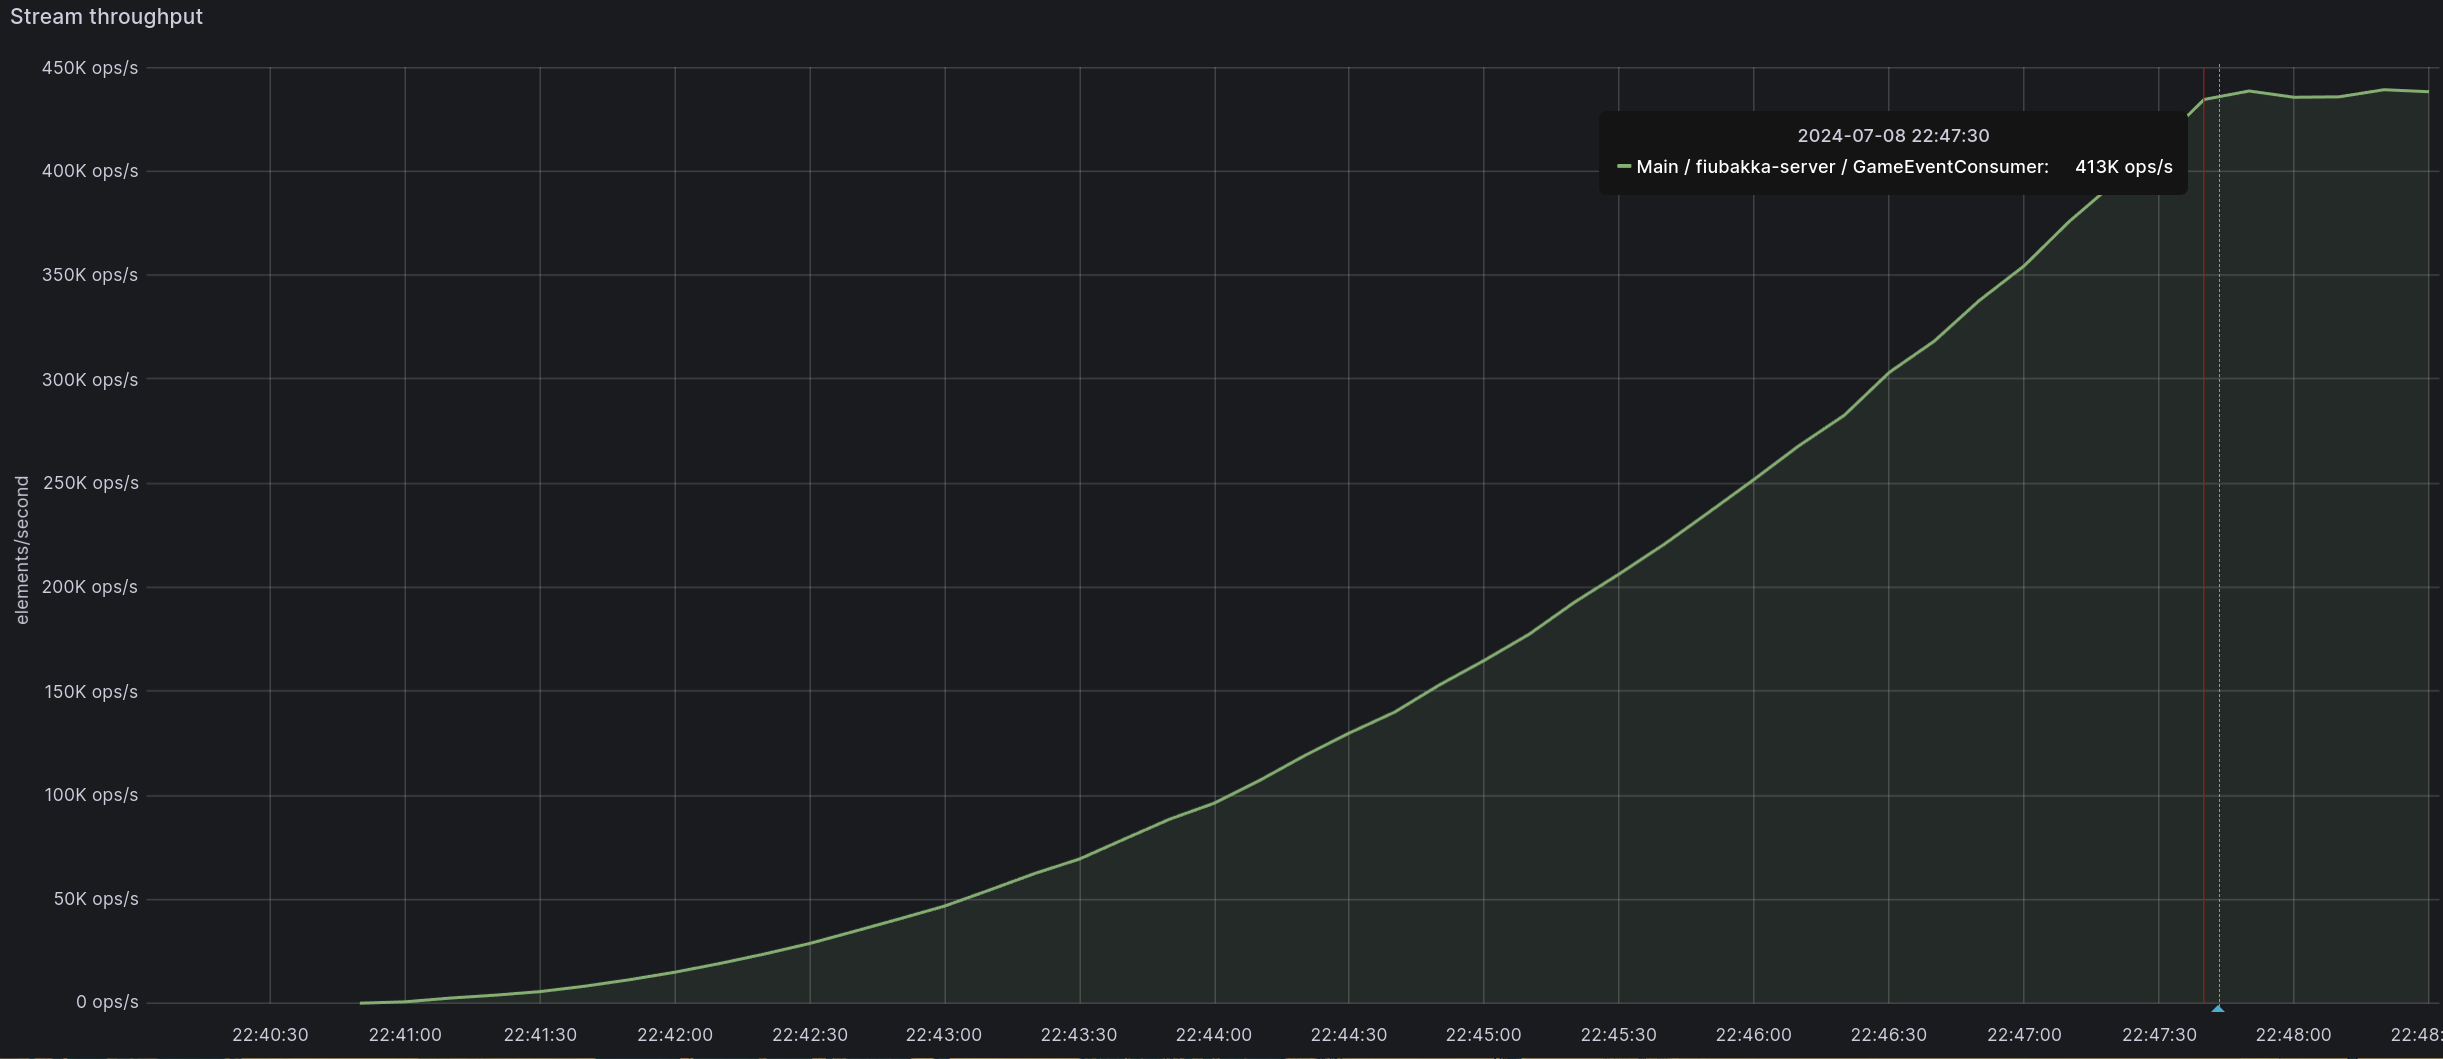
\includegraphics[width=1\textwidth]{../assets/fiubakka-consumer-single-node-metrics.png}
    \caption{Velocidad de consumo de eventos en un único nodo con 84 jugadores.}
\end{figure}

\begin{figure}[htbp]
    \centering
    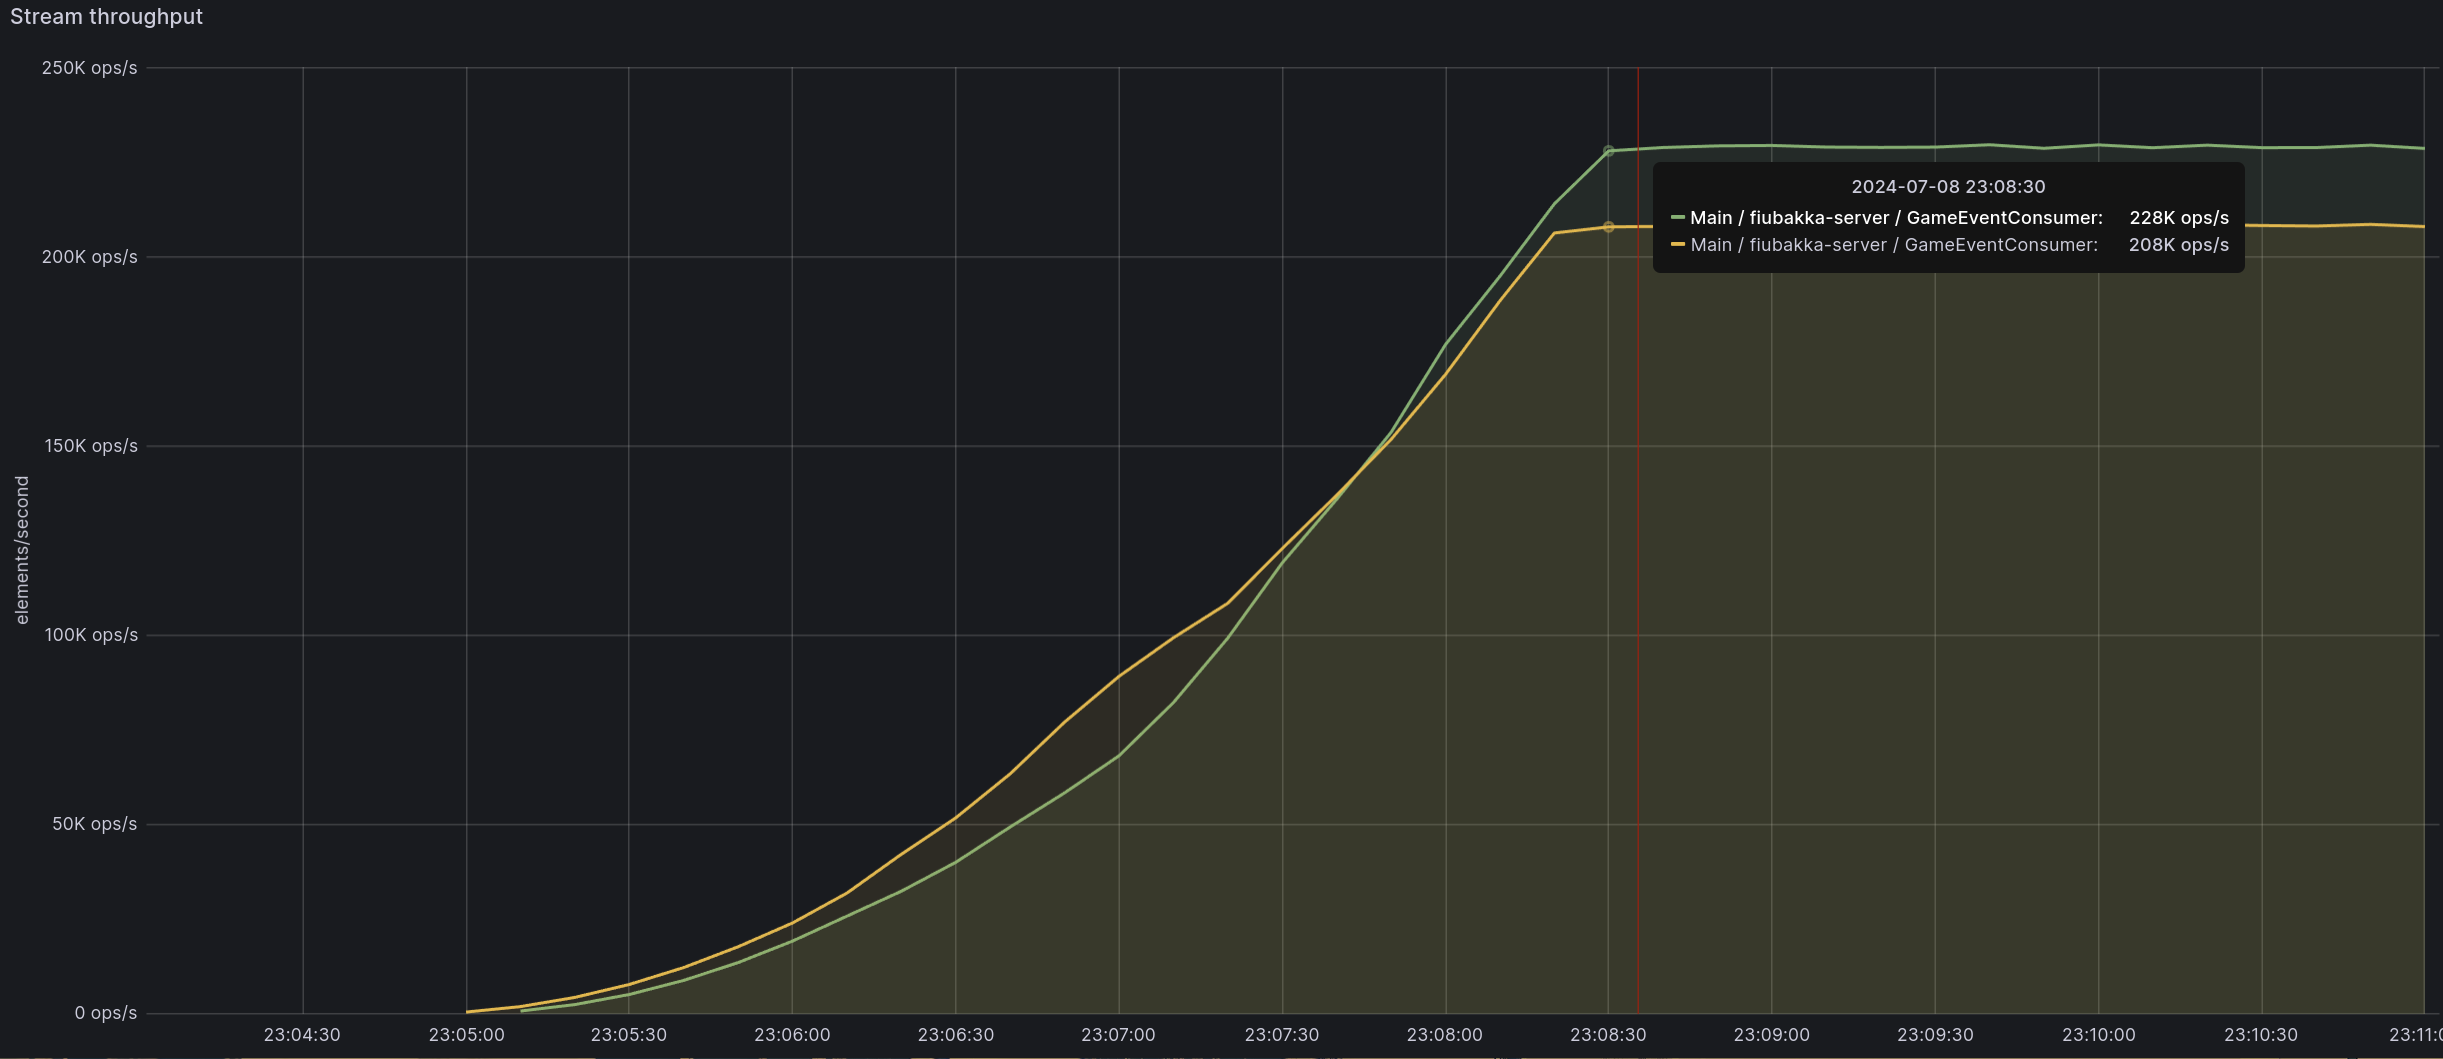
\includegraphics[width=1\textwidth]{../assets/fiubakka-consumer-two-node-metrics.png}
    \caption{Velocidad de consumo de eventos en dos nodos con 84 jugadores en total.}
\end{figure}

\newpage

\begin{figure}[htbp]
    \centering
    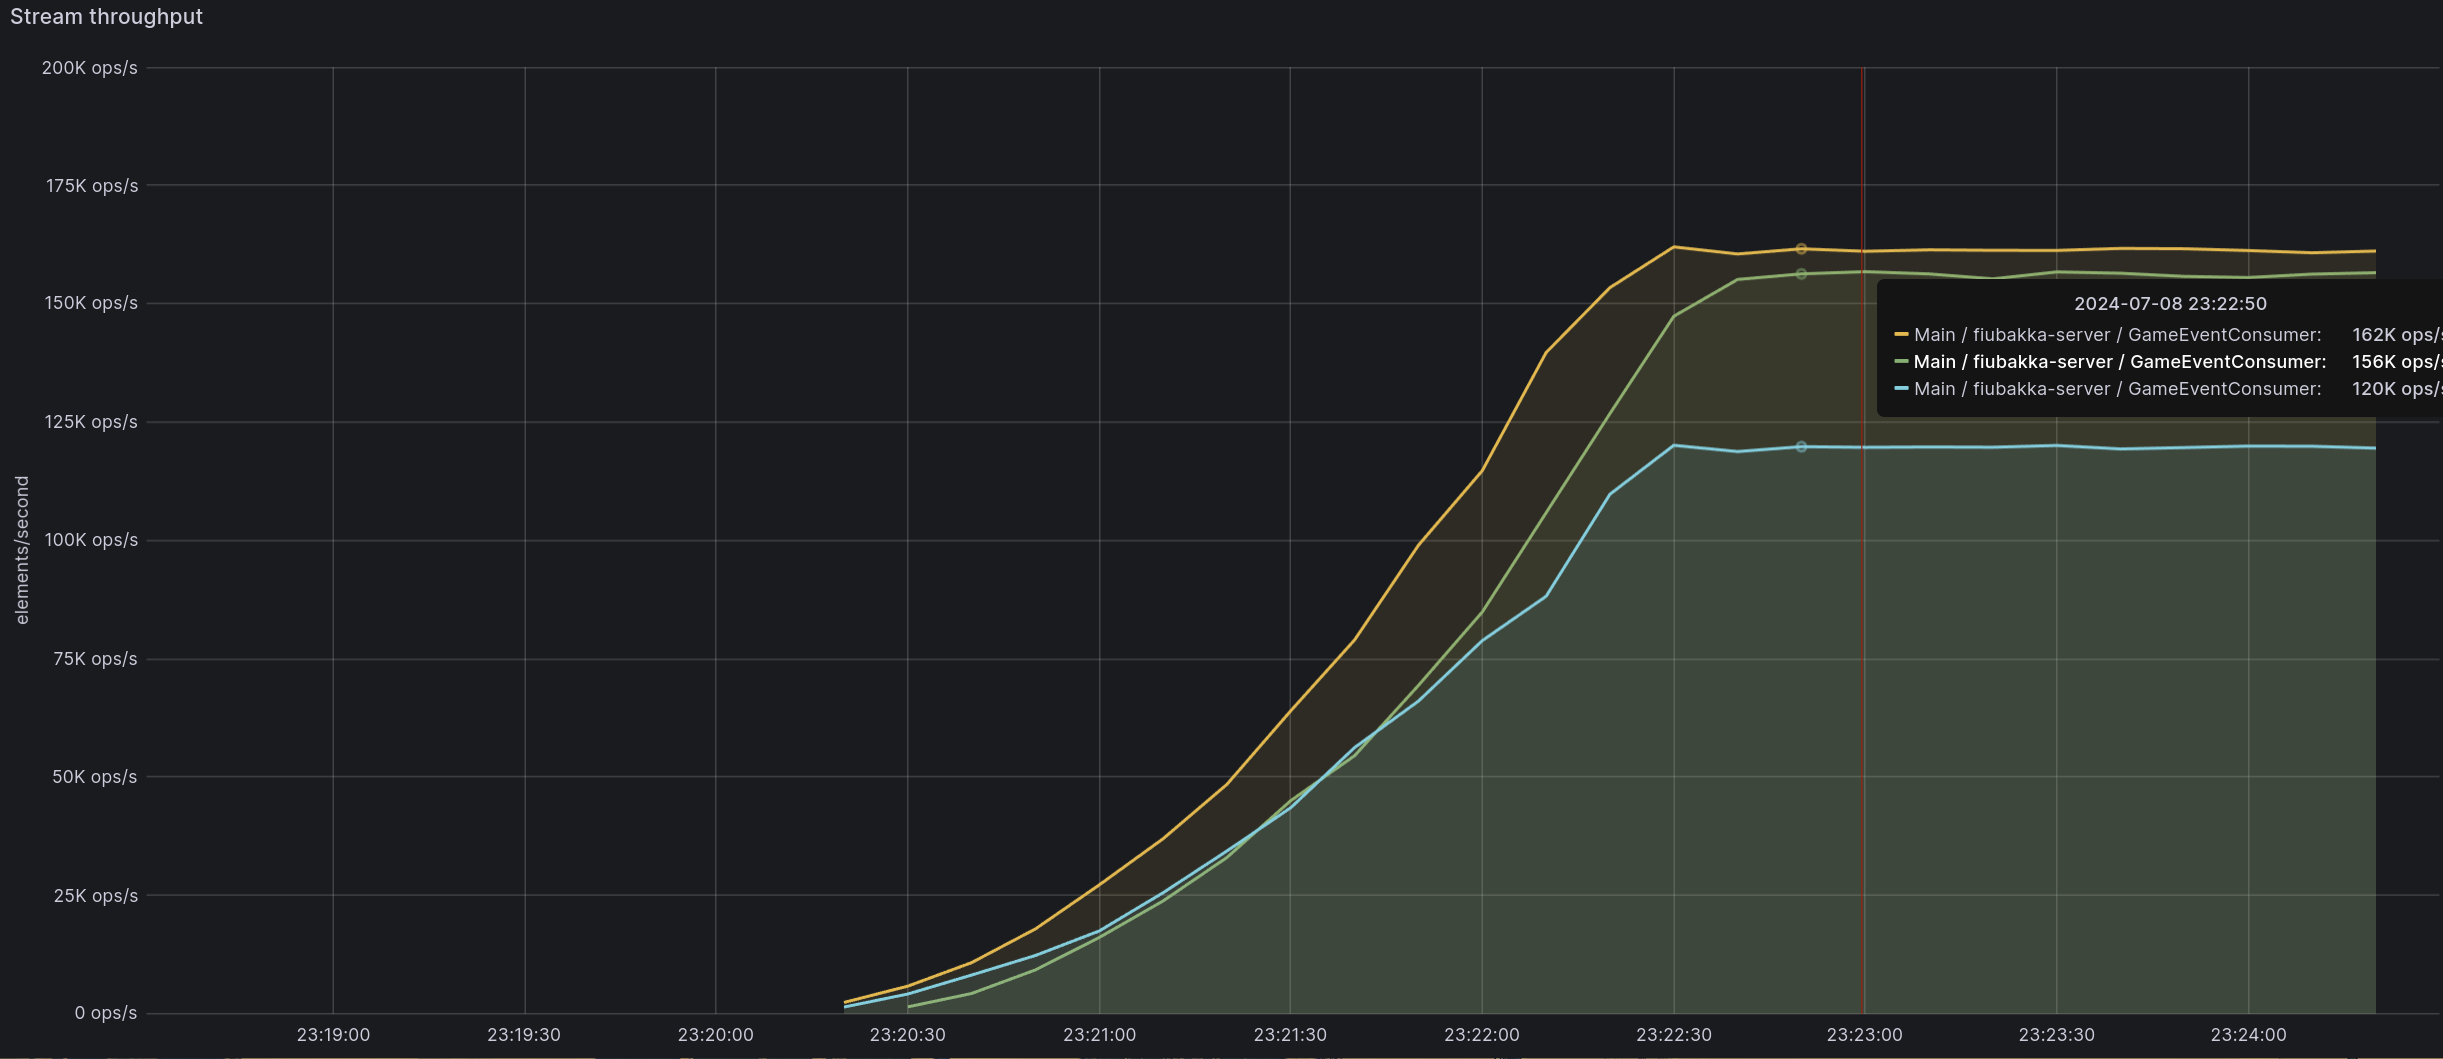
\includegraphics[width=1\textwidth]{../assets/fiubakka-consumer-three-node-metrics.png}
    \caption{Velocidad de consumo de eventos en tres nodos con 84 jugadores en total.}
\end{figure}

Vemos que para los casos de 2 y 3 nodos la carga se distribuye entre ellos de forma equitativa, mantiéndose aproximadamente el mismo valor total de velocidad de consumo de eventos del único nodo si tomamos la suma
de cada velocidad en los casos multinodos. Particularmente, para el caso de 3 nodos se observa que uno de ellos (el celeste) quedó por debajo de los otros. En este caso en particular se dio que algunos jugadores se terminaron procesando
en los otros dos nodos, por lo que la carga del nodo celeste quedo algo por debajo del resto. Los resultados observados coinciden perfectamente con el planteo teórico propuesto anteriormente, y revalidan la hipótestis de escalabilidad
horizontal que planteamos para nuestra arquitectura.

\subsection{Métricas del servidor}

\noindent Ningún sistema está completo sin métricas de monitoreo. Las métricas son esenciales no solo para medir el desempeño de la aplicación, sino también para poder detectar errores y diagnosticar las causas de bajo rendimiento.
\textit{Fiubakka} no es una excepción, y cuenta con una batería de métricas que permiten analizar al detalle la \textit{performance} de cada componente que lo conforma.

Para obtener las métricas de \textit{Fiubakka} utilizamos el plugin de \textbf{Cinnamon}, también conocido como Lightbend Telemetry. Cinnamon es un agente de Java desarrollado por la empresa Lightbend, responsables del desarrollo de tanto Scala
como Akka, para la instrumentación y obtención de métricas de aplicaciones basadas en Akka. Ofrece un conjunto de bibliotecas, todas optativas, para instrumentar cada componente de Akka. Por supuesto, también permite instrumentar la JVM de la aplicación
del nodo.

Los gráficos de métricas de producción y consumición de eventos que mostramos en la secciones anteriores fueron obtenidos mediante Cinnamon, por lo que además resultó ser una herramienta esencial para validar nuestras hipótesis de \textit{performance}
del servidor.

Si bien Cinnamon se encarga de reportar las métricas, es necesario definir un \textit{stack} o conjunto de aplicaciones que nos permitan tanto exportarlas como visualizarlas. Cinnamon cuenta con implementaciones para diversos exportadores de métricas.
En nuestro caso utilizamos \textbf{Prometheus} como servidor de métricas y \textbf{Grafana} como visualizador de las mismas. Prometheus es un servidor de métricas de código abierto que permite almacenar y consultar métricas de forma eficiente.
Mientras que Cinnamon expone un servidor HTTP para consultar las métricas, Prometheus se encarga de \textit{scrapear} el servidor para recolectarlas dada una frecuencia configurada. Grafana se encarga luego de consultar y consumir las métricas almacenadas
en el servidor de Prometheus para visualizarlas en forma de gráficos.

Todas las métricas reportadas por nuestro ambiente productivo pueden ser consultadas en Grafana a través del dominio \textbf{grafana-fiubakka.marcosrolando.uk}. De esta forma tenemos una visión constante y en tiempo real del estado de nuestros servidores de producción.

A continuación se muestran, a modo de ejemplo, tan solo algunos de los distintos gráficos de métricas obtenidas de \textit{Fiubakka}:

\begin{figure}[htbp]
    \centering
    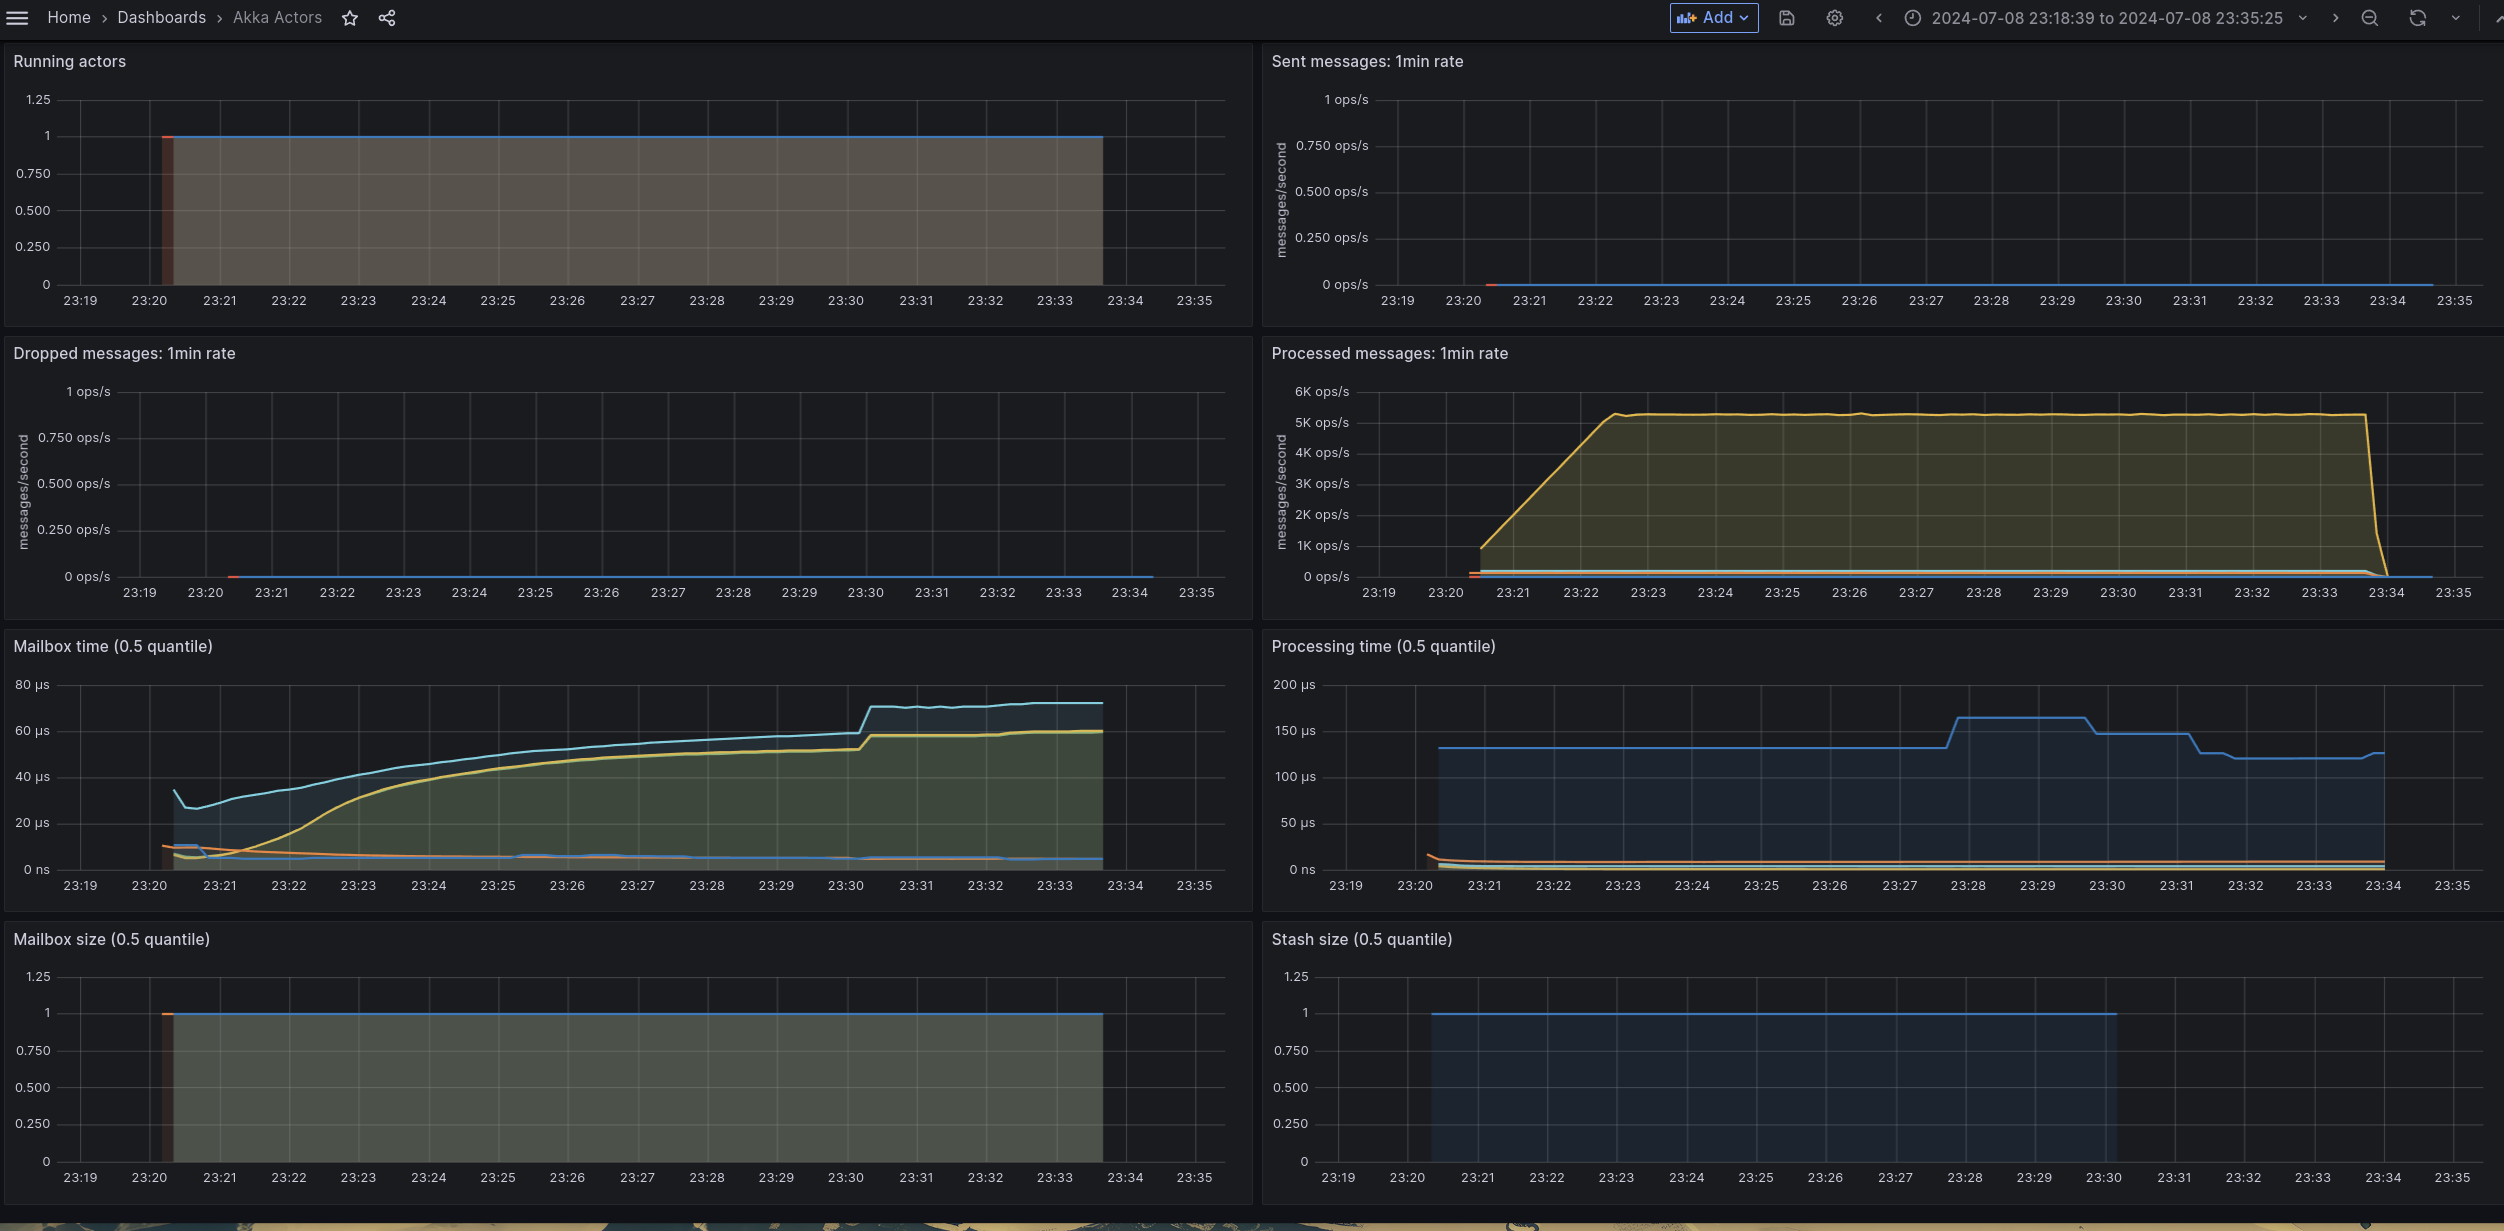
\includegraphics[width=1\textwidth]{../assets/actors-metrics.png}
    \caption{Gráfico de métricas de los actores de \textit{Fiubakka}.}
\end{figure}

\newpage

\begin{figure}[htbp]
    \centering
    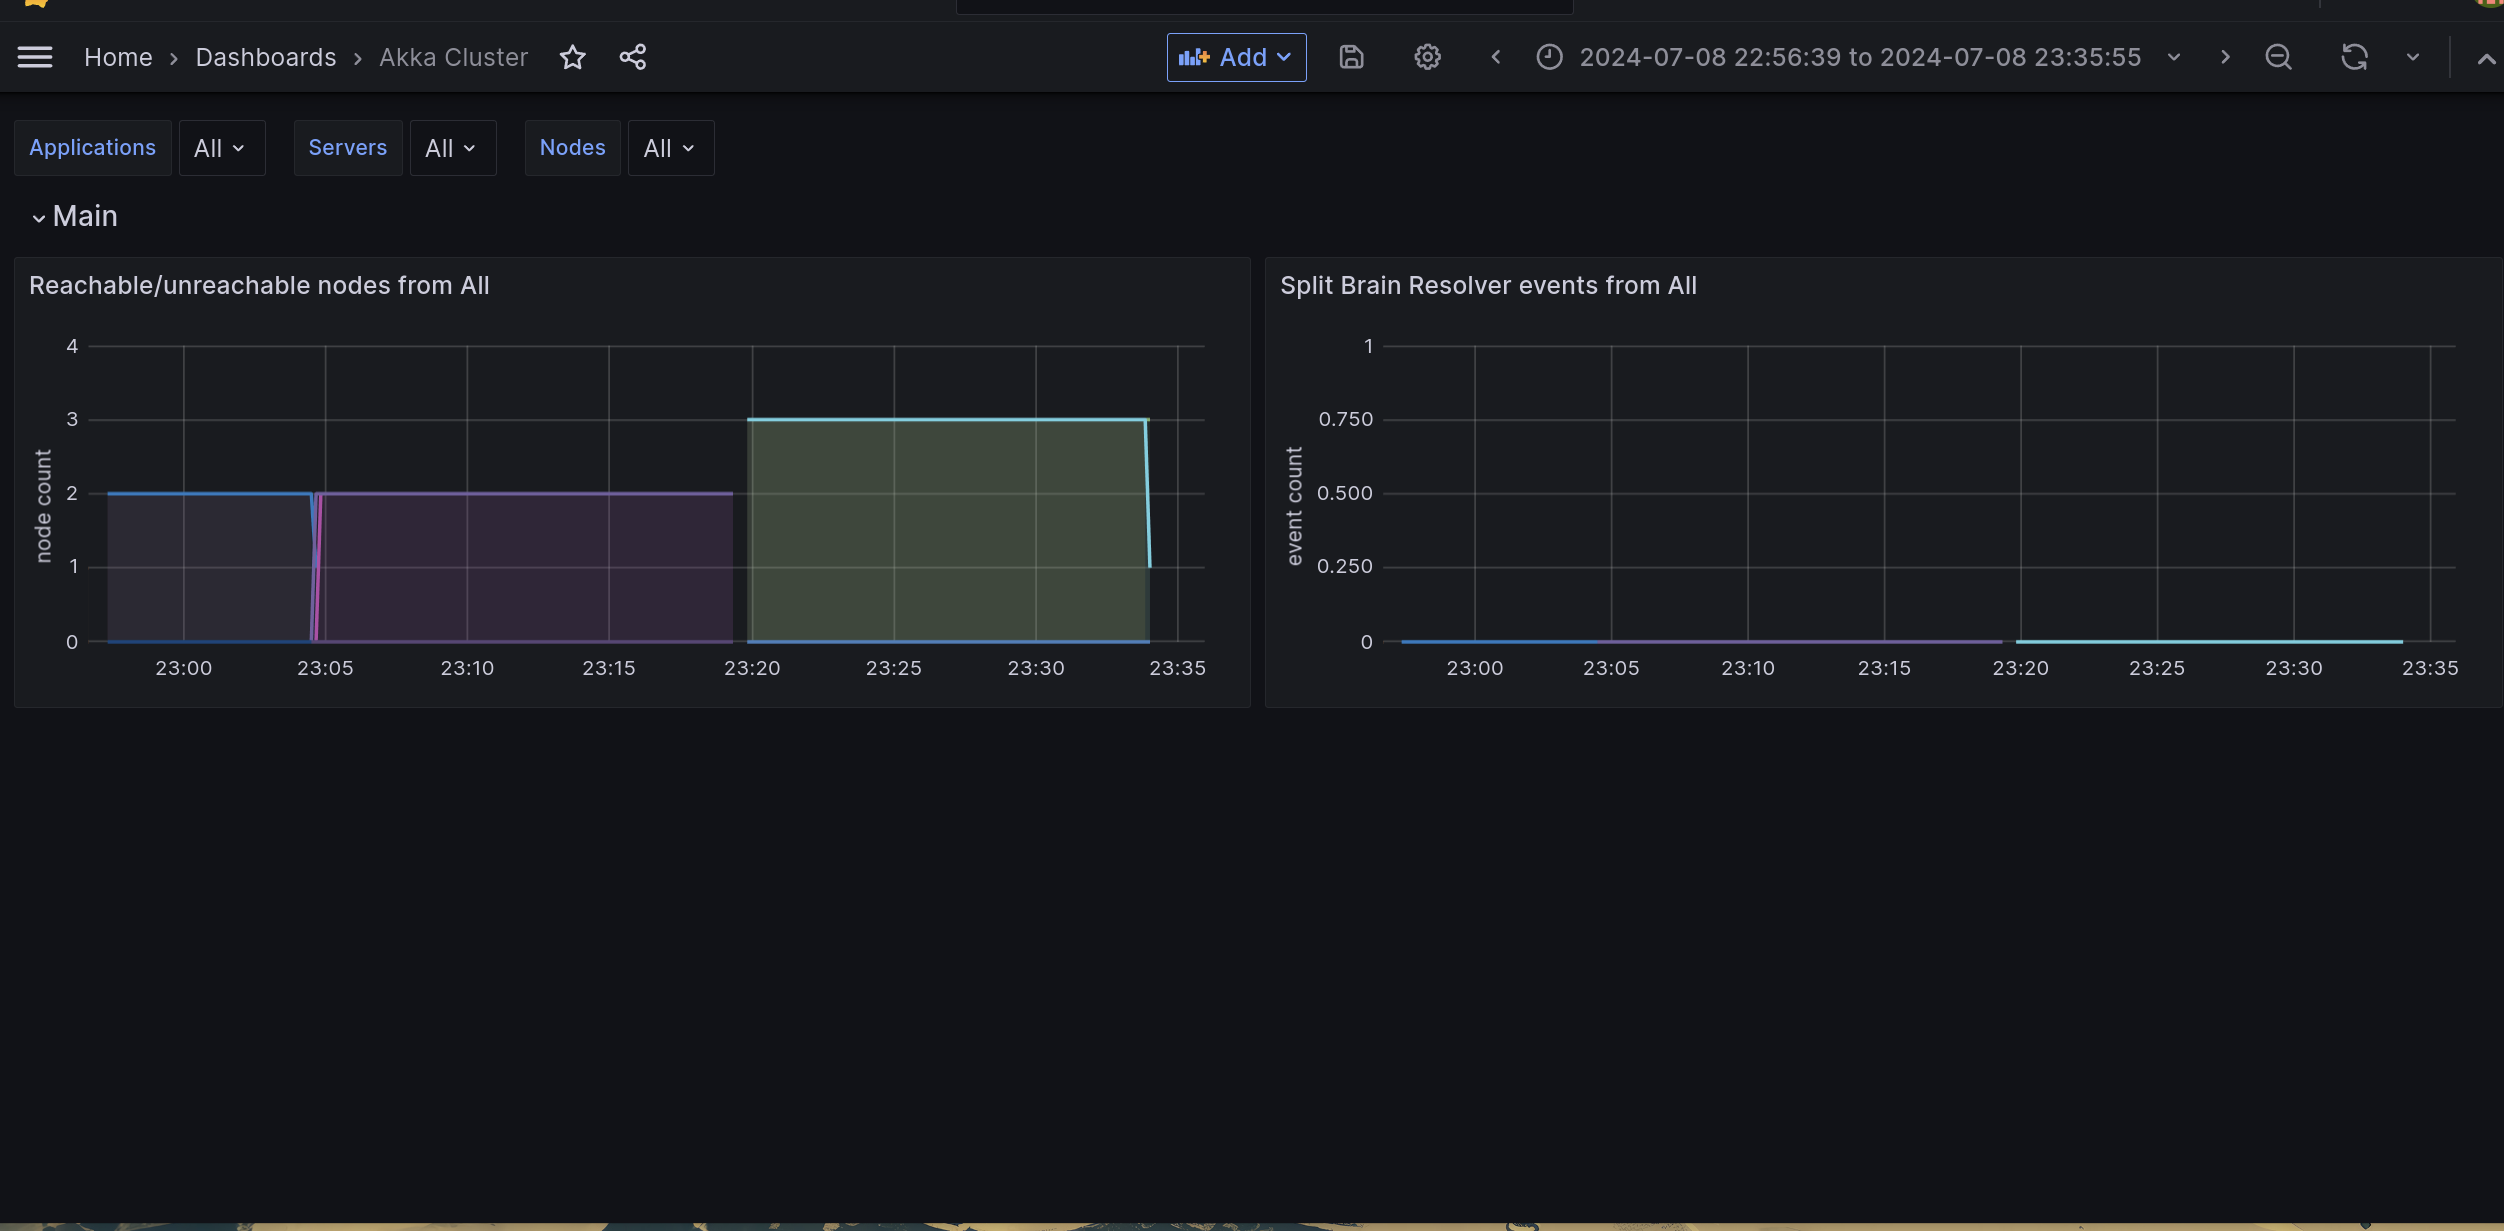
\includegraphics[width=0.9\textwidth]{../assets/cluster-metrics.png}
    \caption{Gráfico de métricas de los nodos del Akka Cluster de \textit{Fiubakka}.}
\end{figure}

\begin{figure}[htbp]
    \centering
    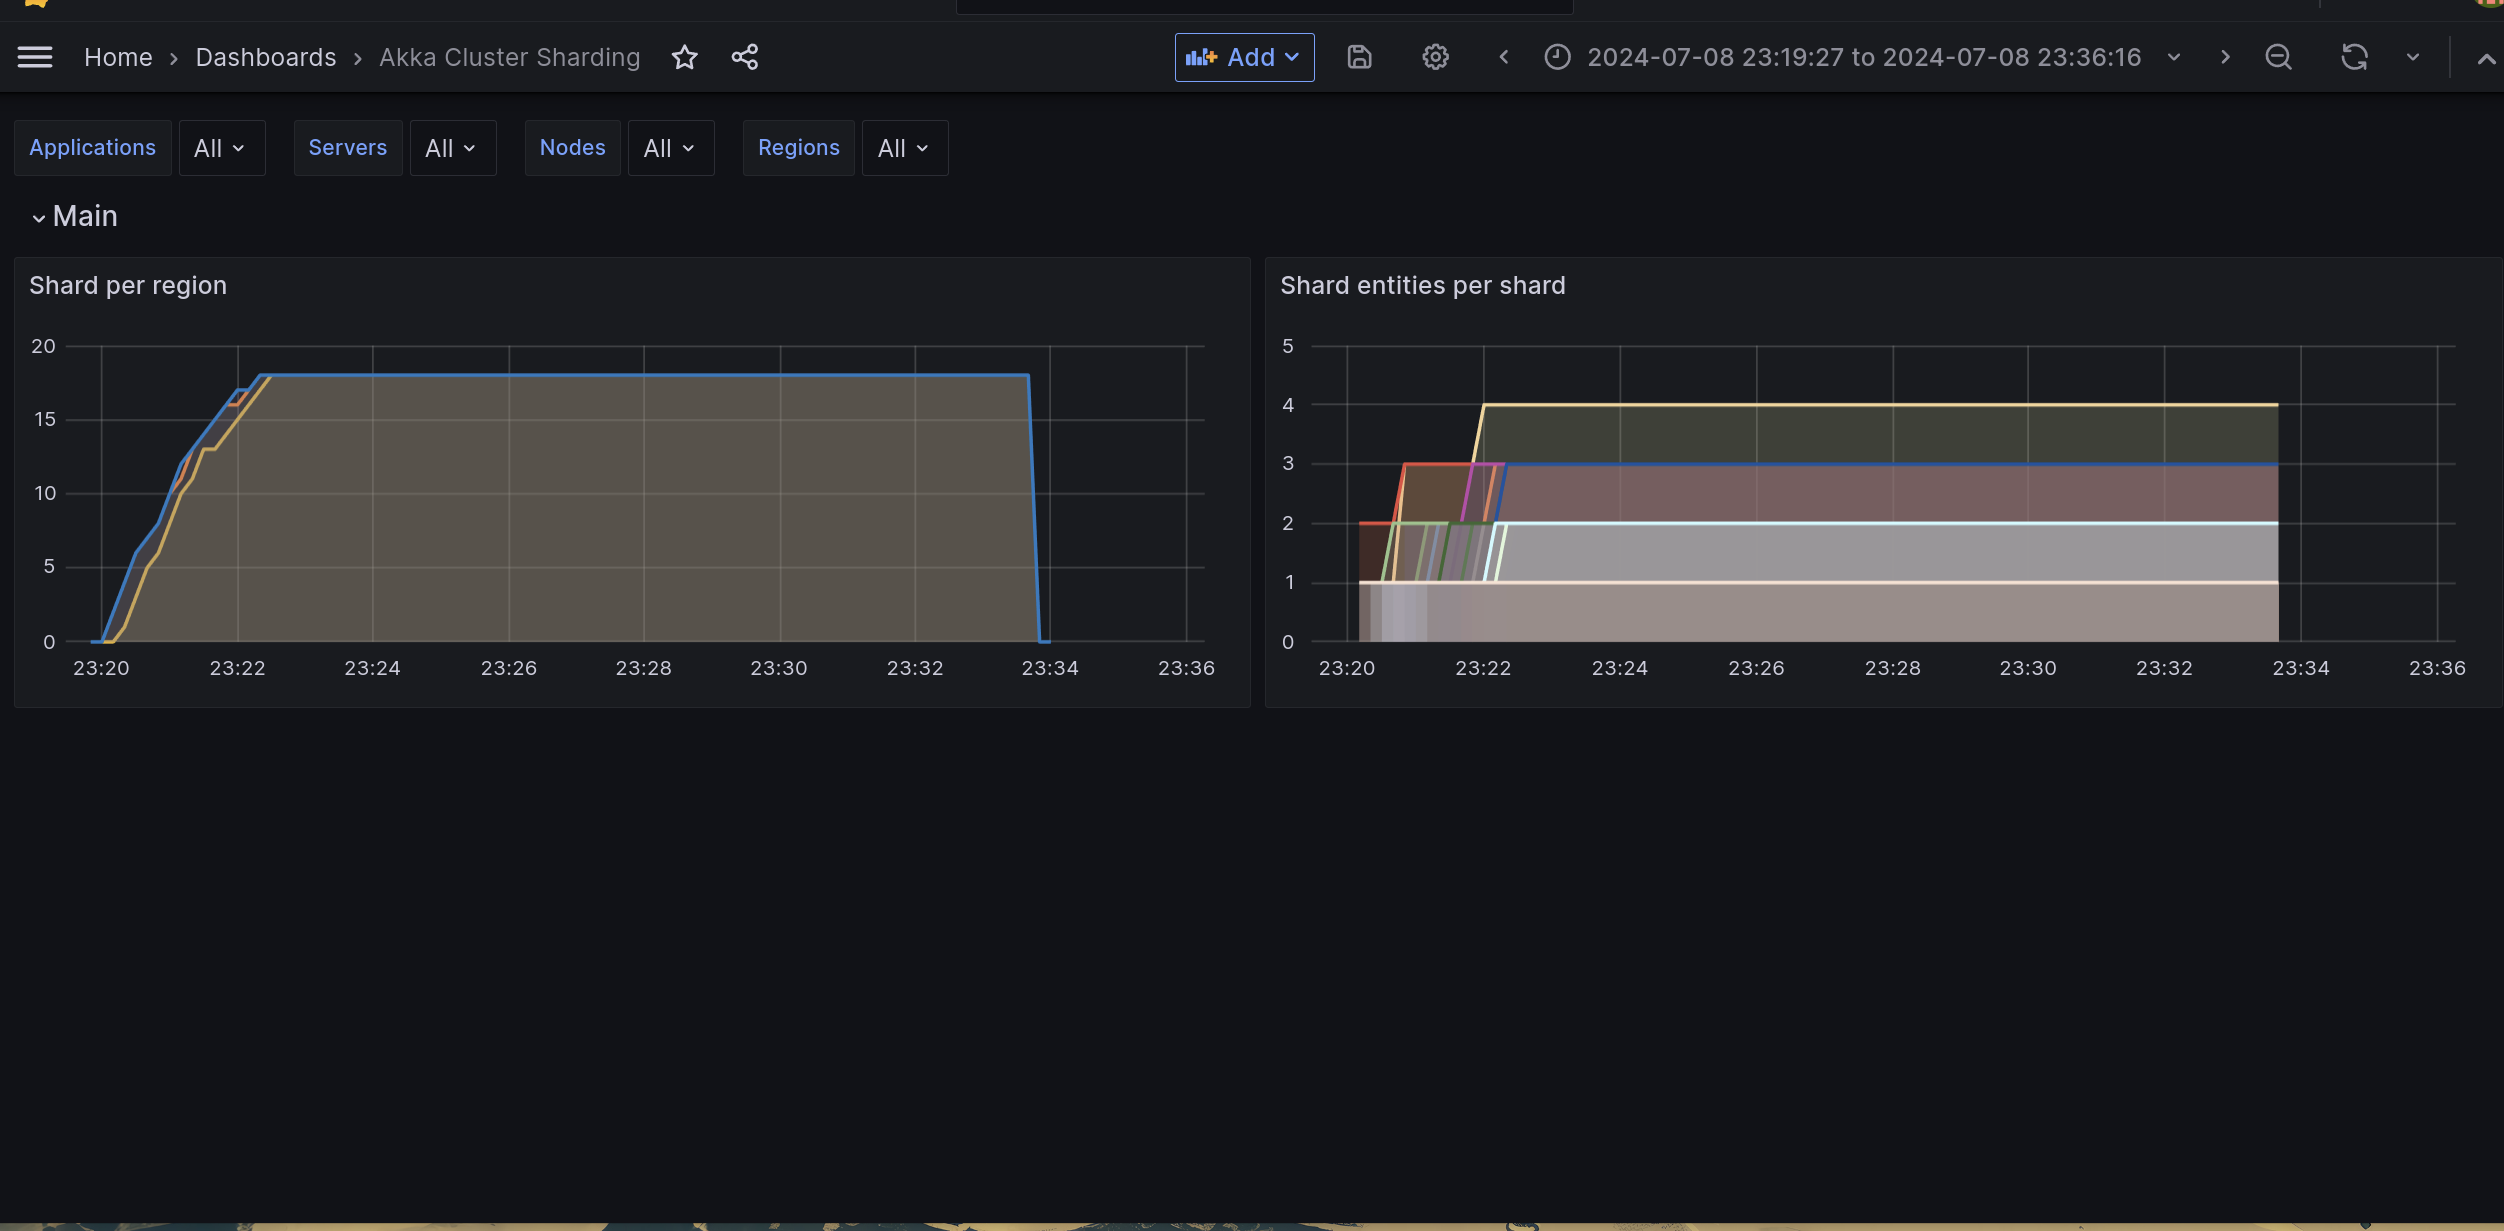
\includegraphics[width=0.9\textwidth]{../assets/cluster-sharding-metrics.png}
    \caption{Gráfico de métricas de Cluster Sharding de \textit{Fiubakka}.}
\end{figure}

\begin{figure}[htbp]
    \centering
    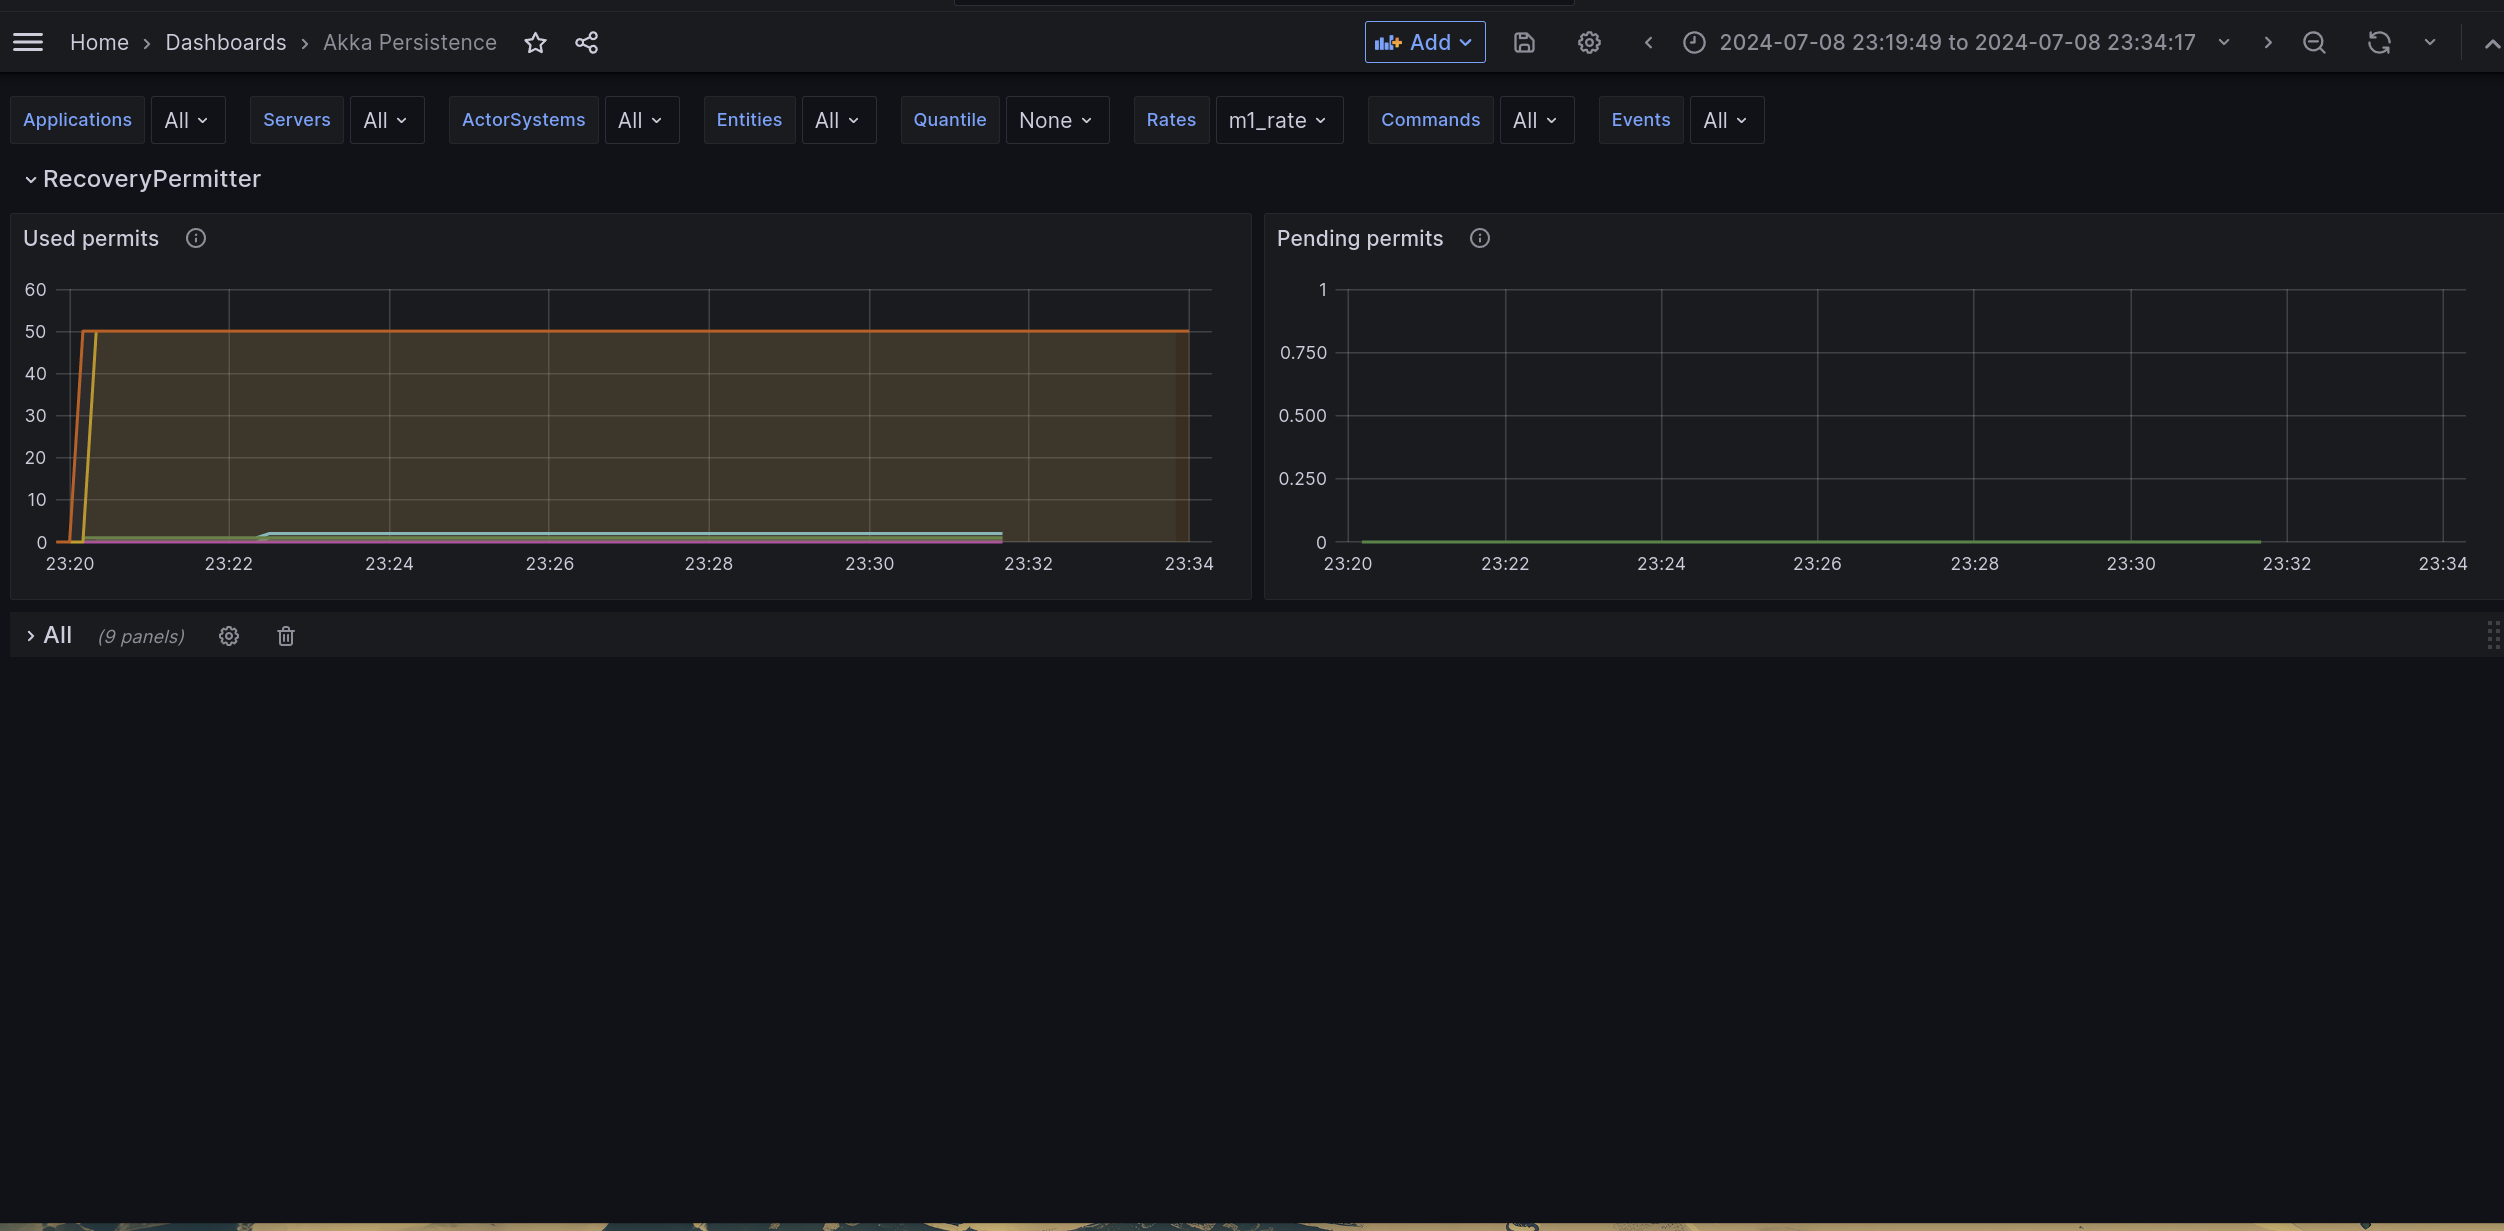
\includegraphics[width=1\textwidth]{../assets/persistence-metrics.png}
    \caption{Gráfico de métricas de Akka Persistence de \textit{Fiubakka}.}
\end{figure}

\begin{figure}[htbp]
    \centering
    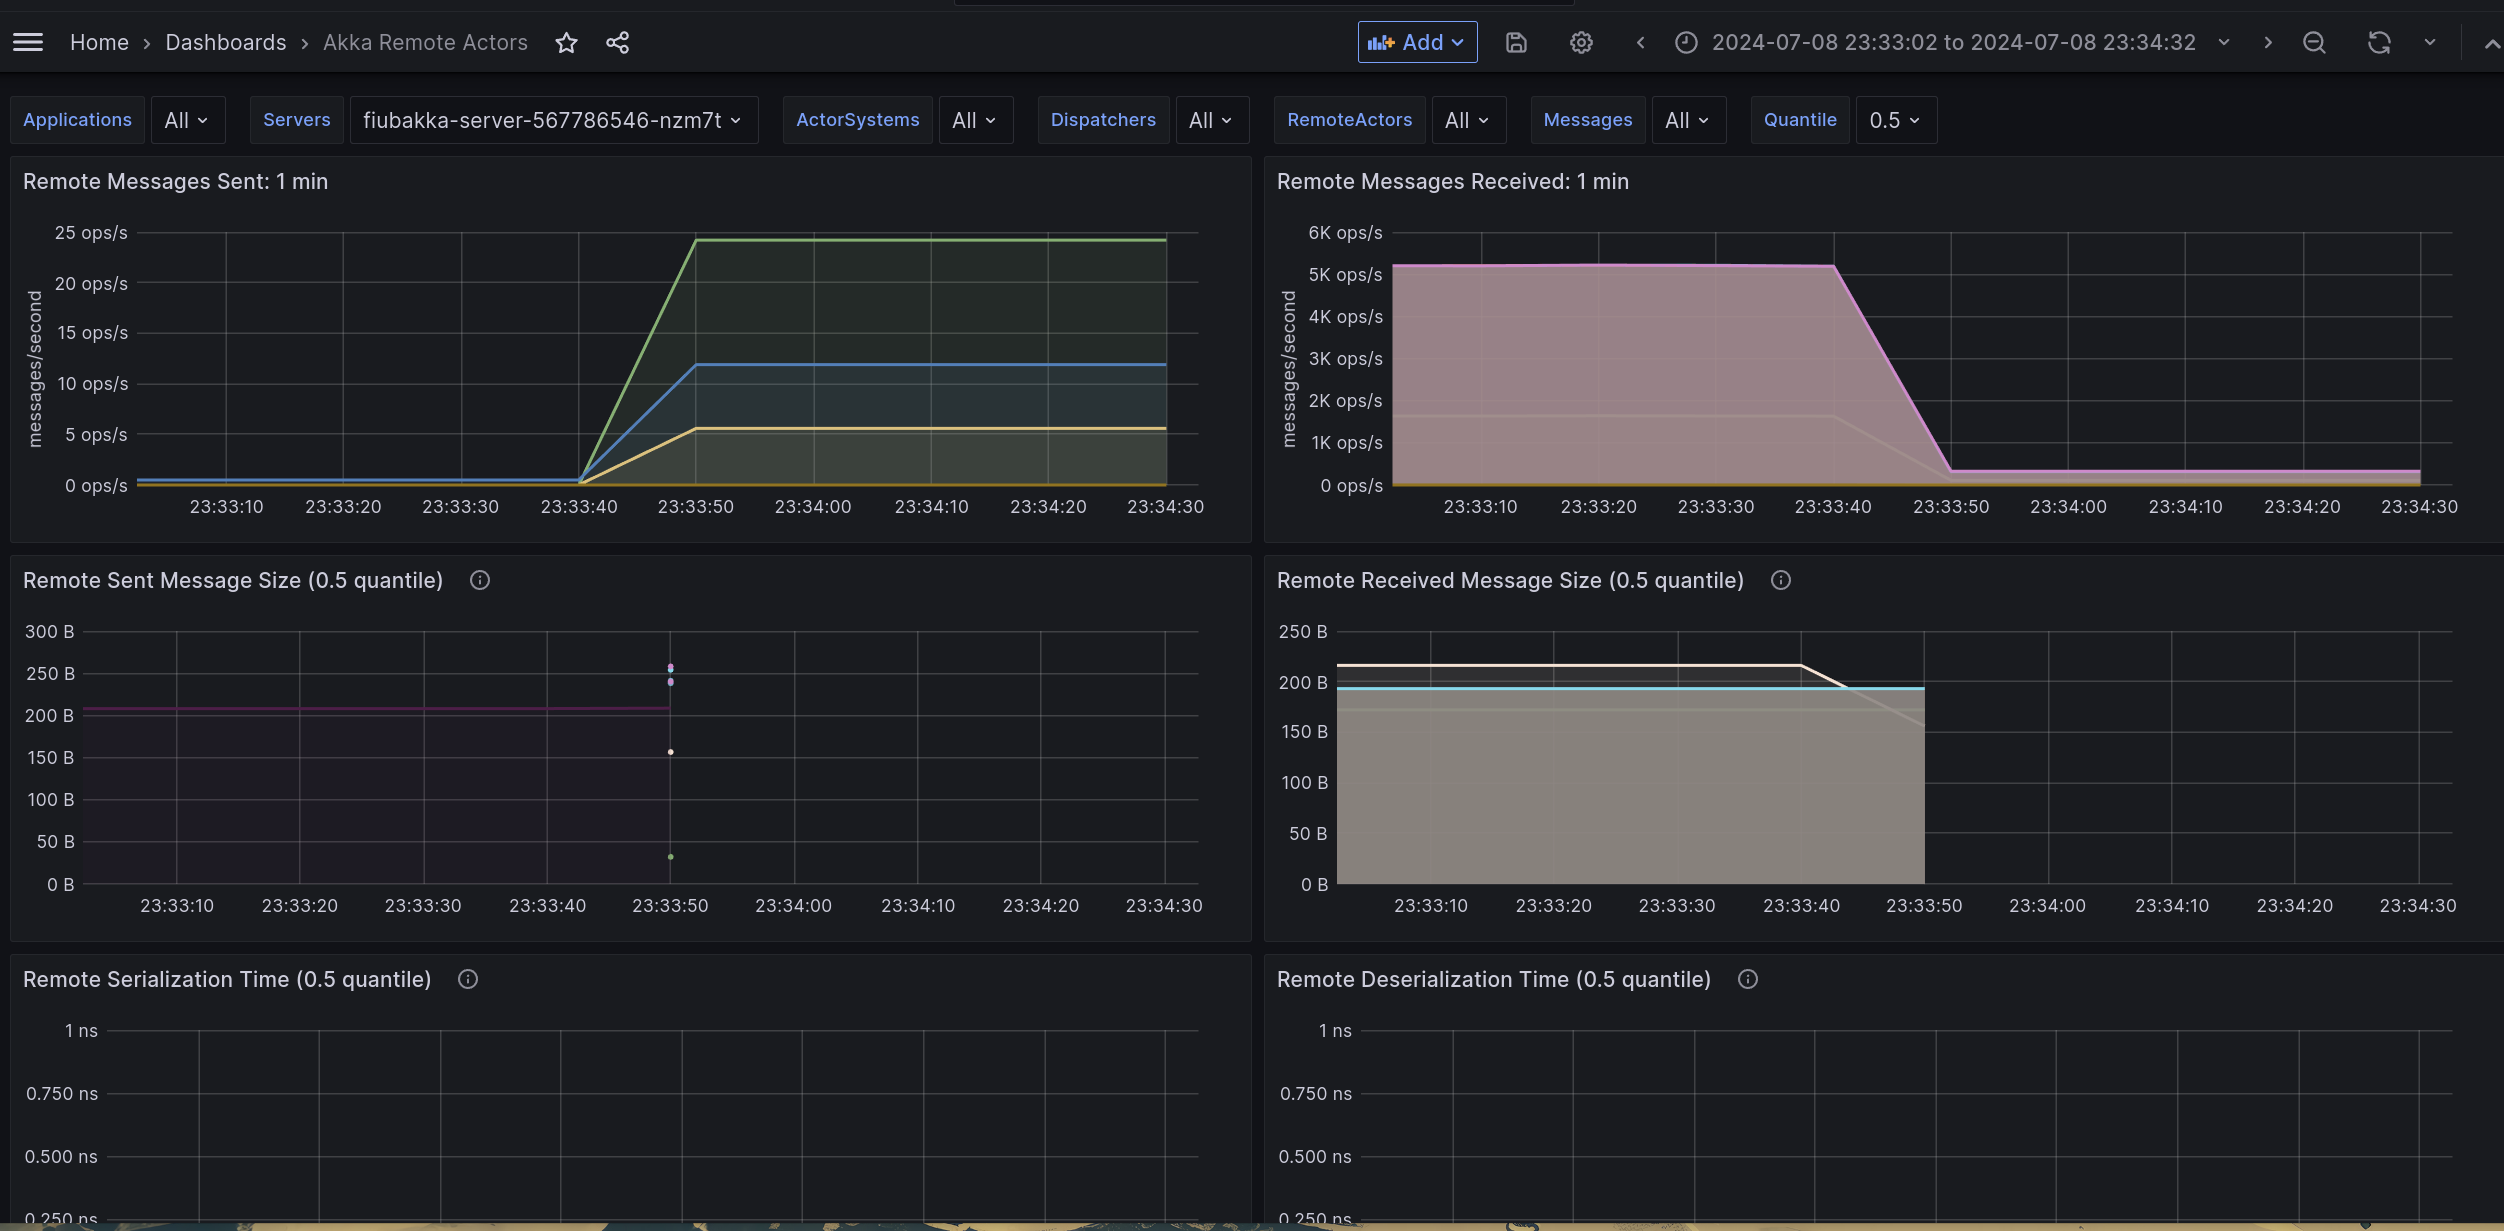
\includegraphics[width=1\textwidth]{../assets/remote-actors-metrics.png}
    \caption{Gráfico de métricas de actores remotos (otros nodos al medido) de \textit{Fiubakka}.}
\end{figure}

\begin{figure}[htbp]
    \centering
    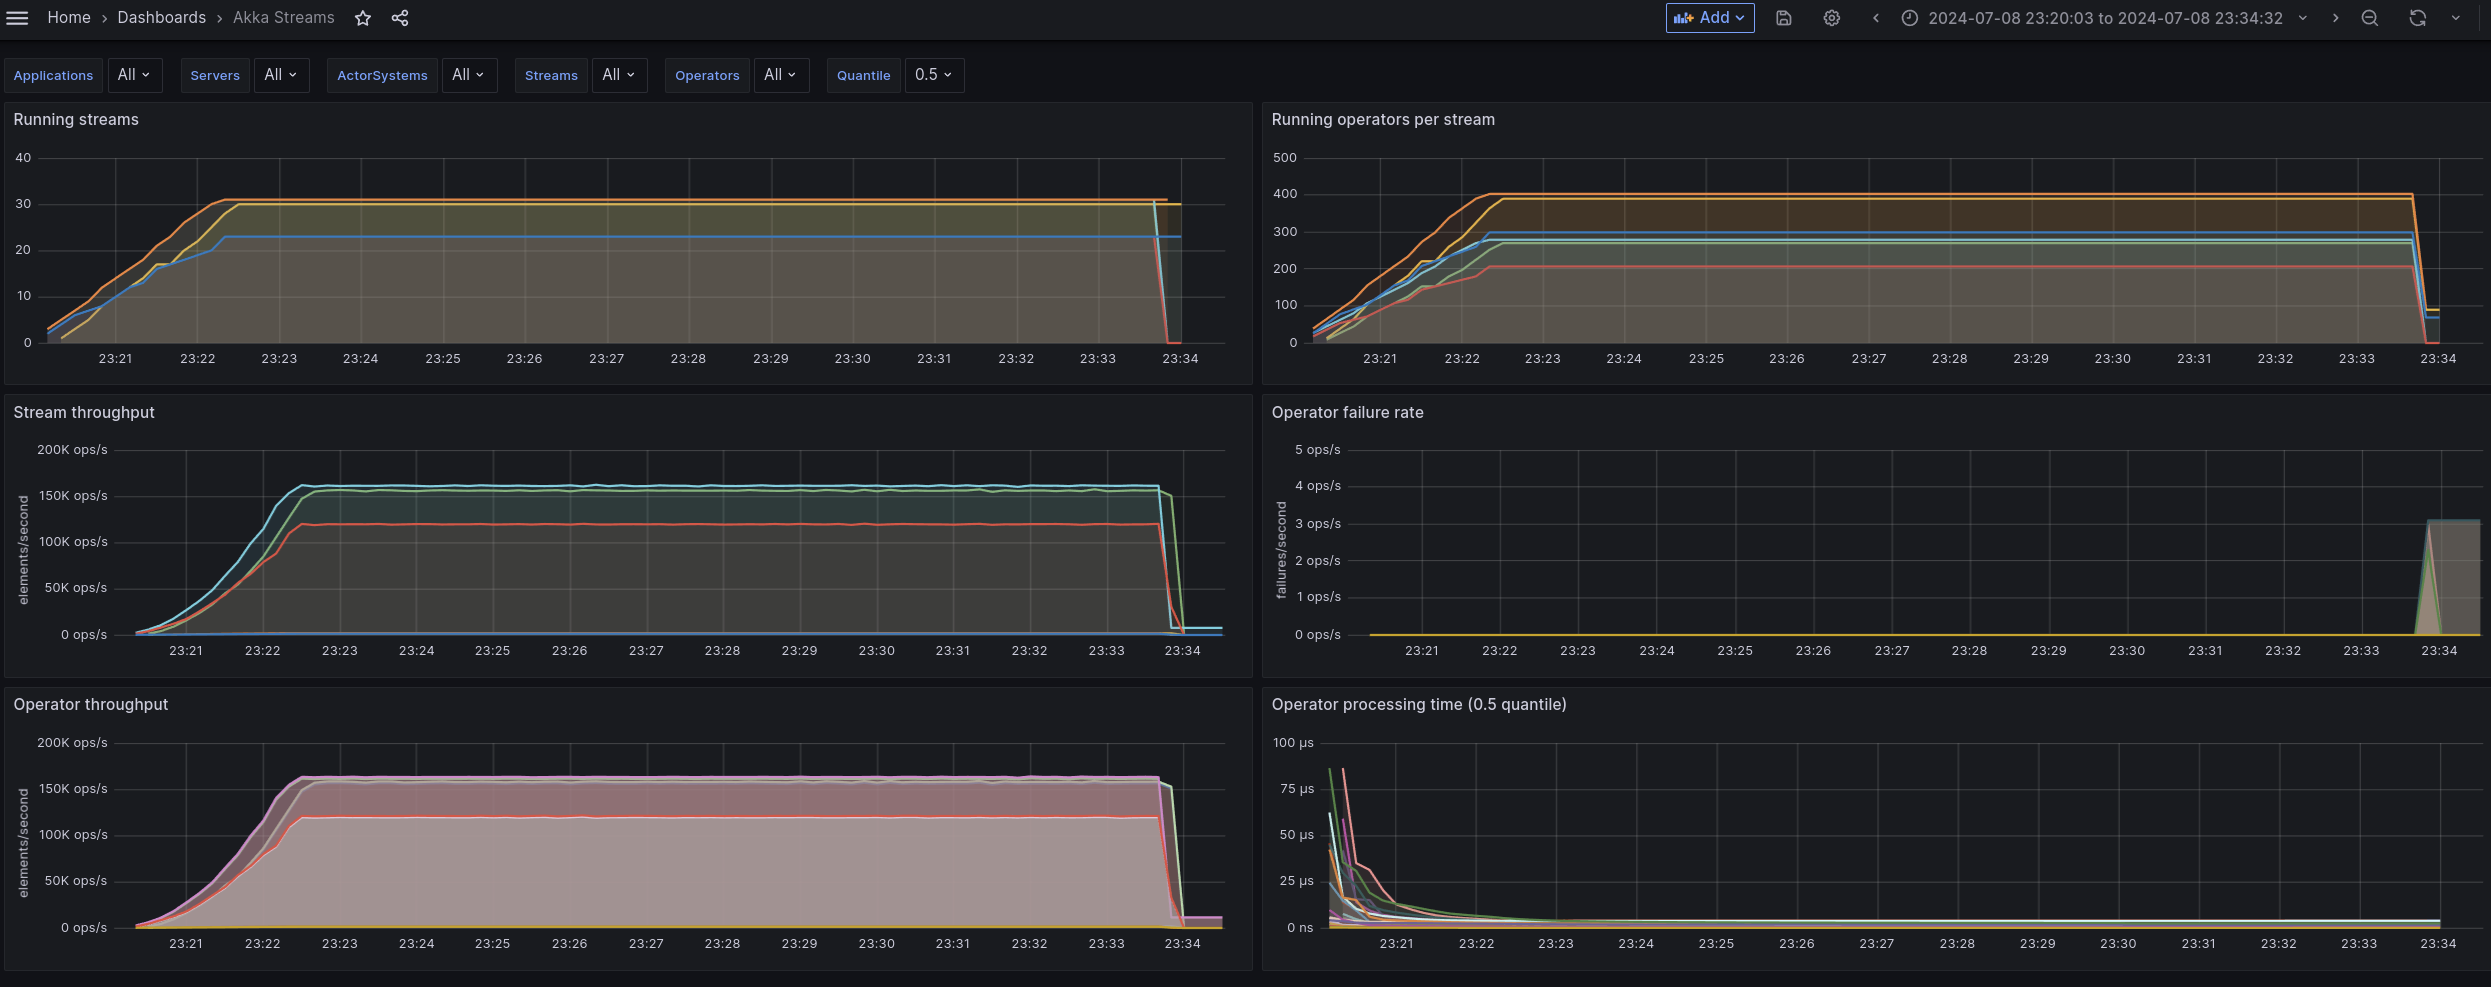
\includegraphics[width=1\textwidth]{../assets/streams-metrics.png}
    \caption{Gráfico de métricas de Akka Streams de \textit{Fiubakka}.}
\end{figure}

\begin{figure}[htbp]
    \centering
    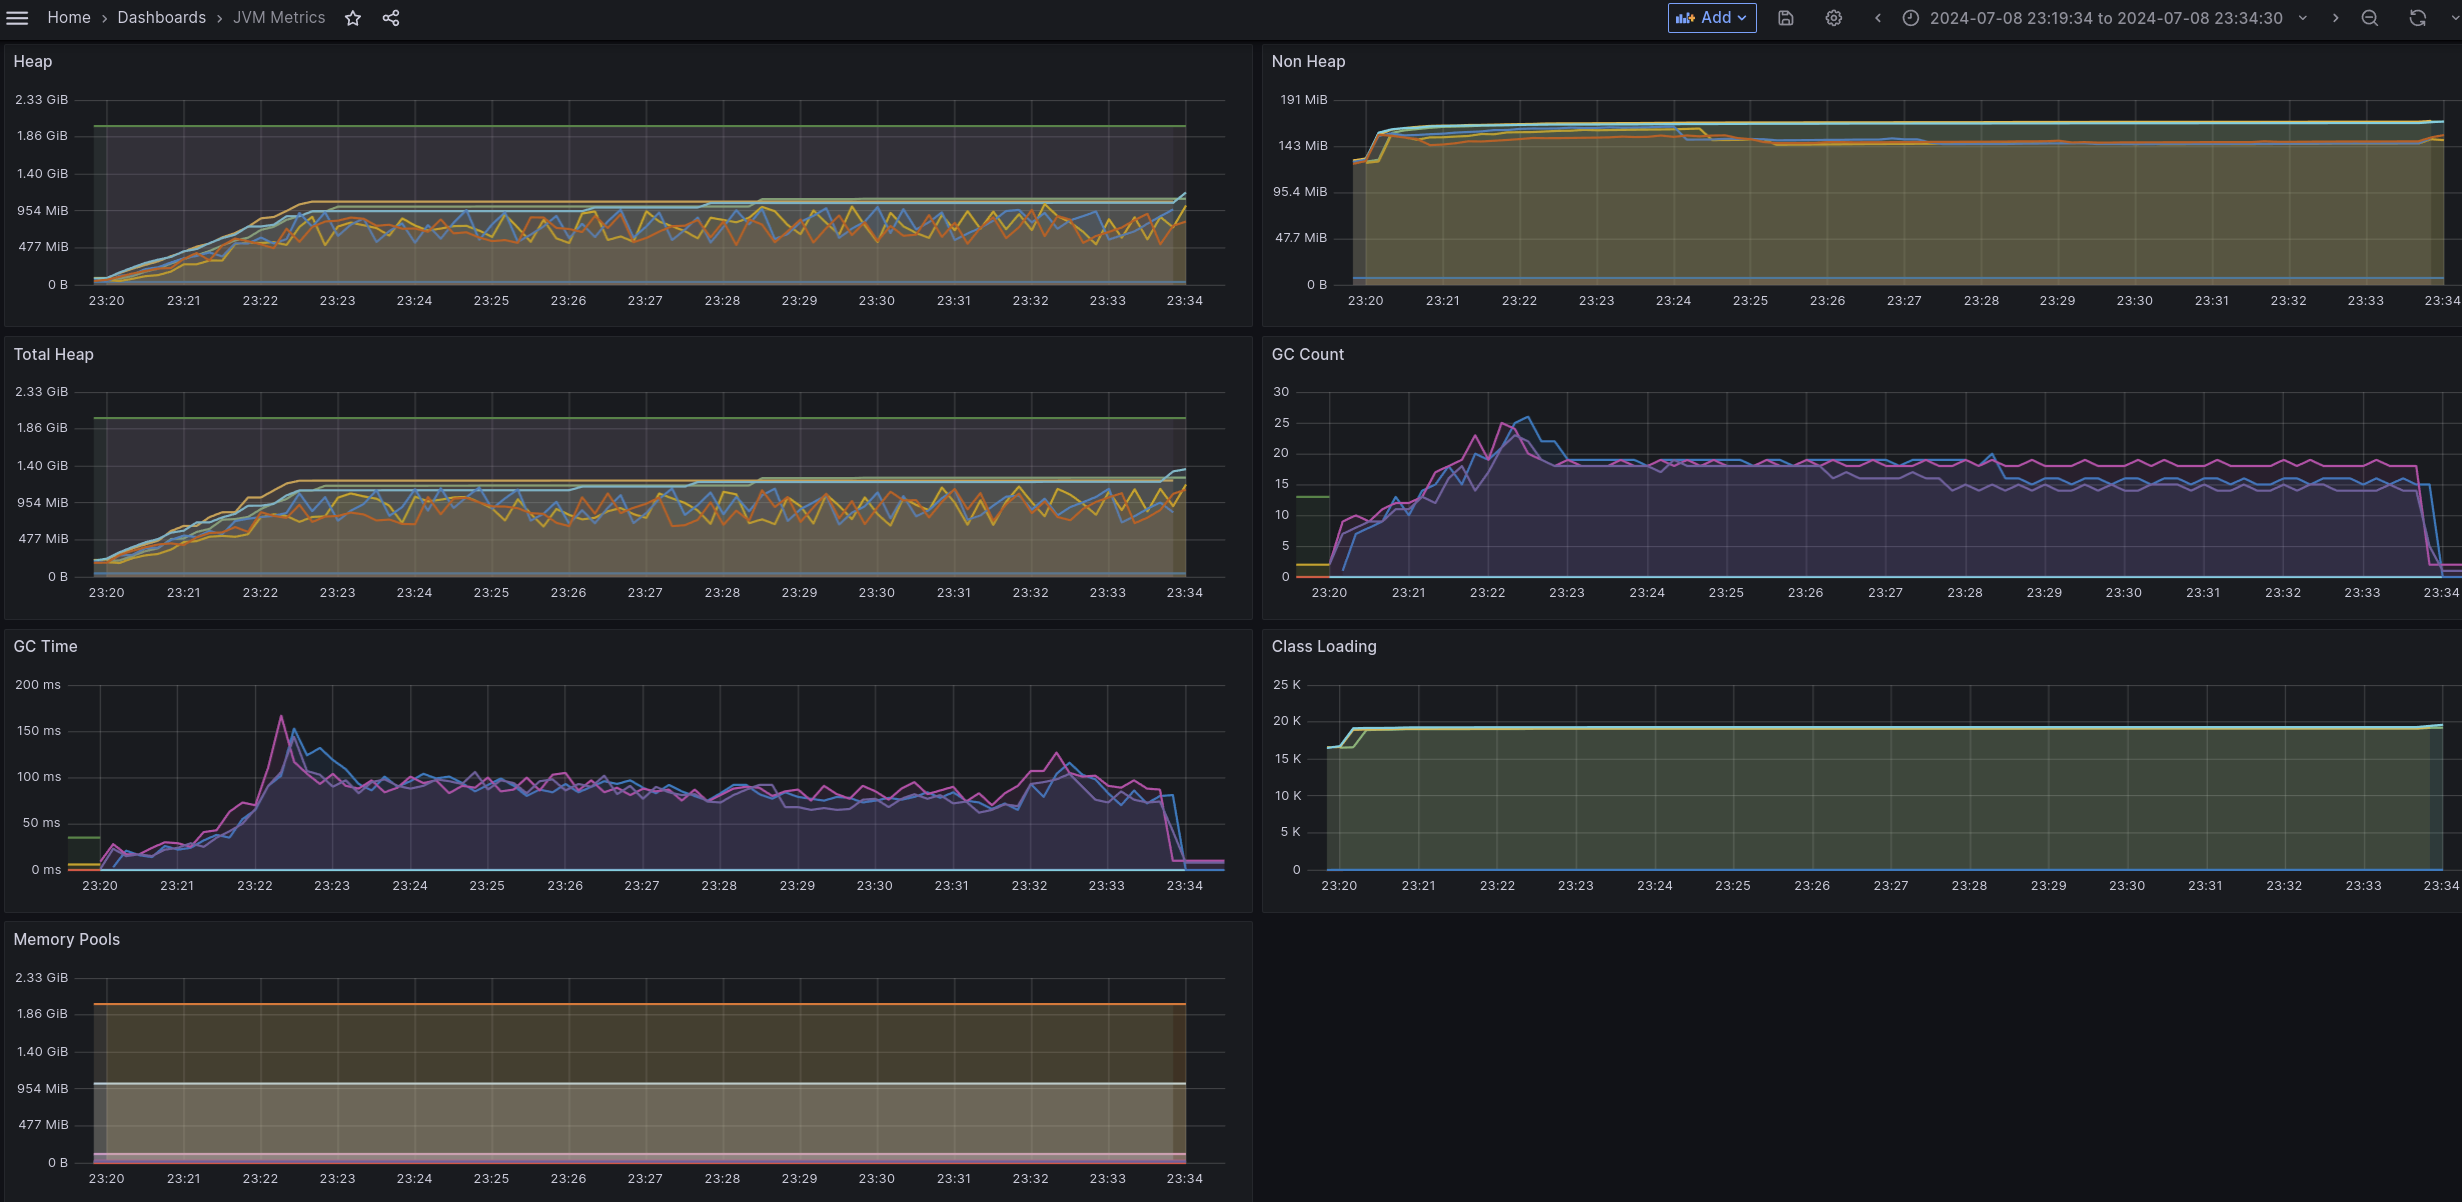
\includegraphics[width=1\textwidth]{../assets/jvm-metrics.png}
    \caption{Gráfico de métricas de las JVMs de los nodos de \textit{Fiubakka}.}
\end{figure}

\newpage

Con esto concluimos el análisis de métricas del servidor. En las siguientes secciones exploraremos las métricas, recursos y requisitos
del cliente del juego.

\subsection{Requisitos del sistema para el cliente del juego}

\noindent Si bien el cliente no es el foco del proyecto, es importante tener en cuenta cuáles son los 
requisitos mínimos del sistema para poder ejecutarlo. Es decir, qué tipo de CPU se necesita,
cuánta capacidad en memoria RAM y cuánto espacio ocupa en disco. Es importante mantener estos requisitos
bajos, para lograr que el juego corra en la mayor cantidad de máquinas posibles y por lo tanto,
que la mayor cantidad de gente pueda jugarlo.

El archivo ejecutable del juego exportado ocupa \textbf{113,7 MB} en Linux y \textbf{115,2 MB} en Windows de memoria en disco.
Es necesario además disponer de al menos \textbf{490 MB} de memoria RAM para ejecutar el juego.
En casos de computadoras sin una placa gráfica dedicada, este requisito de memoria principal puede subir
hasta \textbf{1 GB}, debido a que la VRAM necesaria se consume de la RAM.

Respecto a los requisitos de CPU, estos son más difíciles de medir, debido a que existe una gran cantidad
de modelos de microprocesadores comerciales, cada uno con una combinatoria aún mayor de posibles
configuraciones y rendimientos. Sin embargo, existe una guía en la documentación de Godot \cite{ref3}
con los requisitos mínimos y recomendados para un proyecto 2D o 3D exportado.
Usando esta guía de referencia y teniendo en cuenta que el juego no es muy intensivo en CPU (ya que la mayor parte del tiempo se están enviando y recibiendo paquetes de red), decidimos
tomar como requisito mínimo de CPU el recomendado:

\begin{itemize}
\item \textit{Intel Core 2 Duo E8200}.
\item \textit{AMD Athlon XE BE-2300}.
\end{itemize}

A continuación se confecciona una tabla con todos los requisitos mínimos del sistema. Estos requisitos toman en consideración los recursos consumidos típicamente por el sistema operativo.

\begin{longtable}{|l|l|}
    \hline
    \textbf{CPU} & \textit{Intel Core 2 Duo E8200}.\\
                 & \textit{AMD Athlon XE BE-2300}.\\
    \hline
    \textbf{RAM} & 4 GB.\\
    \hline
    \textbf{Disco rígido} & 32 GB.\\
    \hline
    \textbf{Sistema Operativo} & Sistema operativo Windows o Linux.\\
    \hline
    \caption{Requisitos mínimos del sistema.}\\
\end{longtable}

